% !TeX spellcheck = hu_HU
% !TeX encoding = UTF-8
% !TeX program = xelatex
% TODO Change language to en_GB (recommended) or en_US for English documents
\documentclass[11pt,a4paper,oneside]{report}             % Single-side
%\documentclass[11pt,a4paper,twoside,openright]{report}  % Duplex
\usepackage[utf8]{inputenc}

% thanks to http://tex.stackexchange.com/a/47579/71109
\usepackage{ifxetex}
\usepackage{ifluatex}
\newif\ifxetexorluatex % a new conditional starts as false
\ifnum 0\ifxetex 1\fi\ifluatex 1\fi>0
   \xetexorluatextrue
\fi

\ifxetexorluatex
  \usepackage{fontspec}
\else
  \usepackage[T1]{fontenc}
  \usepackage[utf8]{inputenc}
  \usepackage[lighttt]{lmodern}
\fi

\usepackage[english,magyar]{babel} % Alapértelmezés szerint utoljára definiált nyelv lesz aktív, de később külön beállítjuk az aktív nyelvet.

%\usepackage{cmap}
\usepackage{amsfonts,amsmath,amssymb} % Mathematical symbols.
%\usepackage[ruled,boxed,resetcount,linesnumbered]{algorithm2e} % For pseudocodes. % beware: this is not compatible with LuaLaTeX, see http://tex.stackexchange.com/questions/34814/lualatex-and-algorithm2e
\usepackage{booktabs} % For publication quality tables for LaTeX
\usepackage{graphicx}

%\usepackage{fancyhdr}
%\usepackage{lastpage}

\usepackage{anysize}
%\usepackage{sectsty}
\usepackage{setspace} % For setting line spacing

\usepackage[unicode]{hyperref} % For hyperlinks in the generated document.
\usepackage{xcolor}
\usepackage{listings} % For source code snippets.

\usepackage[amsmath,thmmarks]{ntheorem} % Theorem-like environments.

\usepackage[hang]{caption}

\singlespacing

\newcommand{\selecthungarian}{
	\selectlanguage{magyar}
	\setlength{\parindent}{2em}
	\setlength{\parskip}{0em}
	\frenchspacing
}

\newcommand{\selectenglish}{
	\selectlanguage{english}
	\setlength{\parindent}{0em}
	\setlength{\parskip}{0.5em}
	\nonfrenchspacing
	\renewcommand{\figureautorefname}{Figure}
	\renewcommand{\tableautorefname}{Table}
	\renewcommand{\partautorefname}{Part}
	\renewcommand{\chapterautorefname}{Chapter}
	\renewcommand{\sectionautorefname}{Section}
	\renewcommand{\subsectionautorefname}{Section}
	\renewcommand{\subsubsectionautorefname}{Section}
}

\usepackage[numbers]{natbib}
\usepackage{xspace}
\def\UrlBreaks{\do\/\do-} % URL törés '-' mentén

%TODO Set the main variables
\newcommand{\vikszerzoVezeteknev}{Madarász}
\newcommand{\vikszerzoKeresztnev}{Bence}

\newcommand{\vikkonzulensAMegszolitas}{}
\newcommand{\vikkonzulensAVezeteknev}{Kövesdán}
\newcommand{\vikkonzulensAKeresztnev}{Gábor}

\newcommand{\vikkonzulensBMegszolitas}{}
\newcommand{\vikkonzulensBVezeteknev}{}
\newcommand{\vikkonzulensBKeresztnev}{}

\newcommand{\vikkonzulensCMegszolitas}{}
\newcommand{\vikkonzulensCVezeteknev}{}
\newcommand{\vikkonzulensCKeresztnev}{}

\newcommand{\vikcim}{Continuous Deployment és elasztikus skálázás megvalósítása
webalkalmazásokhoz} % Cím
\newcommand{\viktanszek}{\bmeaut} % Tanszék
\newcommand{\vikdoktipus}{\bsc} % Dokumentum típusa (\bsc vagy \msc)
\newcommand{\vikmunkatipusat}{szakdolgozatot} % a "hallgató nyilatkozat" részhez: szakdolgozatot vagy diplomatervet

%--------------------------------------------------------------------------------------
% TDK-specifikus változók
%--------------------------------------------------------------------------------------
\newcommand{\tdkszerzoB}{Második Szerző} % Második szerző neve; hagyd üresen, ha egyedül írtad a TDK-t.
\newcommand{\tdkev}{2014} % A dolgozat írásának éve (pl. "2014") (Ez OTDK-nál eltérhet az aktuális évtől.)

% További adatok az OTDK címlaphoz (BME-s TDK-hoz nem kell kitölteni)
\newcommand{\tdkevfolyamA}{IV} % Első szerző évfolyama, római számmal (pl. IV).
\newcommand{\tdkevfolyamB}{III} % Második szerző évfolyama, római számmal (pl. III).
\newcommand{\tdkkonzulensbeosztasA}{egyetemi tanár} % Első konzulens beosztása (pl. egyetemi docens)
\newcommand{\tdkkonzulensbeosztasB}{doktorandusz} % Második konzulens beosztása (pl. egyetemi docens)

\newcommand{\szerzoMeta}{\vikszerzoVezeteknev{} \vikszerzoKeresztnev} % egy szerző esetén
%\newcommand{\szerzoMeta}{\vikszerzoVezeteknev{} \vikszerzoKeresztnev, \tdkszerzoB} % két szerző esetén

%TODO Language configuration -- choose one
% Beállítások magyar nyelvű dolgozathoz
%--------------------------------------------------------------------------------------
% Elnevezések
%--------------------------------------------------------------------------------------
\newcommand{\bme}{Budapesti Műszaki és Gazdaságtudományi Egyetem}
\newcommand{\vik}{Villamosmérnöki és Informatikai Kar}

\newcommand{\bmemit}{Méréstechnika és Információs Rendszerek Tanszék}
\newcommand{\bmeaut}{Automatizálási és Alkalmazott Informatikai Tanszék}

\newcommand{\keszitette}{Készítette}
\newcommand{\konzulens}{Konzulens}

\newcommand{\bsc}{Szakdolgozat}
\newcommand{\msc}{Diplomaterv}
\newcommand{\tdk}{TDK dolgozat}
\newcommand{\bsconlab}{BSc Önálló laboratórium}
\newcommand{\msconlabi}{MSc Önálló laboratórium 1.}
\newcommand{\msconlabii}{MSc Önálló laboratórium 2.}

\newcommand{\pelda}{Példa}
\newcommand{\definicio}{Definíció}
\newcommand{\tetel}{Tétel}

\newcommand{\bevezetes}{Bevezetés}
\newcommand{\koszonetnyilvanitas}{Köszönetnyilvánítás}
\newcommand{\fuggelek}{Függelék}

% Opcionálisan átnevezhető címek
%\addto\captionsmagyar{%
%\renewcommand{\listfigurename}{Saját ábrajegyzék cím}
%\renewcommand{\listtablename}{Saját táblázatjegyzék cím}
%\renewcommand{\bibname}{Saját irodalomjegyzék név}
%}

\newcommand{\szerzo}{\vikszerzoVezeteknev{} \vikszerzoKeresztnev}
\newcommand{\vikkonzulensA}{\vikkonzulensAMegszolitas\vikkonzulensAVezeteknev{} \vikkonzulensAKeresztnev}
\newcommand{\vikkonzulensB}{\vikkonzulensBMegszolitas\vikkonzulensBVezeteknev{} \vikkonzulensBKeresztnev}
\newcommand{\vikkonzulensC}{\vikkonzulensCMegszolitas\vikkonzulensCVezeteknev{} \vikkonzulensCKeresztnev}

\newcommand{\selectthesislanguage}{\selecthungarian}

\bibliographystyle{huplain}

\def\lstlistingname{lista}

\newcommand{\appendixnumber}{6}  % a fofejezet-szamlalo az angol ABC 6. betuje (F) lesz

% Settings for English documents
%%--------------------------------------------------------------------------------------
% Elnevezések
%--------------------------------------------------------------------------------------
\newcommand{\bme}{Budapest University of Technology and Economics}
\newcommand{\vik}{Faculty of Electrical Engineering and Informatics}

\newcommand{\bmemit}{Department of Measurement and Information Systems}

\newcommand{\keszitette}{Author}
\newcommand{\konzulens}{Advisor}

\newcommand{\bsc}{Bachelor's Thesis}
\newcommand{\msc}{Master's Thesis}
\newcommand{\tdk}{Scientific Students' Association Report}
\newcommand{\bsconlab}{BSc Project Laboratory}
\newcommand{\msconlabi}{MSc Project Laboratory 1}
\newcommand{\msconlabii}{MSc Project Laboratory 2}

\newcommand{\pelda}{Example}
\newcommand{\definicio}{Definition}
\newcommand{\tetel}{Theorem}

\newcommand{\bevezetes}{Introduction}
\newcommand{\koszonetnyilvanitas}{Acknowledgements}
\newcommand{\fuggelek}{Appendix}

% Optional custom titles
%\addto\captionsenglish{%
%\renewcommand*{\listfigurename}{Your list of figures title}
%\renewcommand*{\listtablename}{Your list of tables title}
%\renewcommand*{\bibname}{Your bibliography title}
%}

\newcommand{\szerzo}{\vikszerzoKeresztnev{} \vikszerzoVezeteknev}
\newcommand{\vikkonzulensA}{\vikkonzulensAMegszolitas\vikkonzulensAKeresztnev{} \vikkonzulensAVezeteknev}
\newcommand{\vikkonzulensB}{\vikkonzulensBMegszolitas\vikkonzulensBKeresztnev{} \vikkonzulensBVezeteknev}
\newcommand{\vikkonzulensC}{\vikkonzulensCMegszolitas\vikkonzulensCKeresztnev{} \vikkonzulensCVezeteknev}

\newcommand{\selectthesislanguage}{\selectenglish}

\bibliographystyle{plainnat}

\newcommand{\ie}{i.e.\@\xspace}
\newcommand{\Ie}{I.e.\@\xspace}
\newcommand{\eg}{e.g.\@\xspace}
\newcommand{\Eg}{E.g.\@\xspace}
\newcommand{\etal}{et al.\@\xspace}
\newcommand{\etc}{etc.\@\xspace}
\newcommand{\vs}{vs.\@\xspace}
\newcommand{\viz}{viz.\@\xspace} % videlicet
\newcommand{\cf}{cf.\@\xspace} % confer
\newcommand{\Cf}{Cf.\@\xspace}
\newcommand{\wrt}{w.r.t.\@\xspace} % with respect to
\newcommand{\approximately}{approx.\@\xspace}

\newcommand{\appendixnumber}{1}  % a fofejezet-szamlalo az angol ABC 1. betuje (A) lesz


%--------------------------------------------------------------------------------------
% Page layout setup
%--------------------------------------------------------------------------------------
% we need to redefine the pagestyle plain
% another possibility is to use the body of this command without \fancypagestyle
% and use \pagestyle{fancy} but in that case the special pages
% (like the ToC, the References, and the Chapter pages)remain in plane style

\pagestyle{plain}
\marginsize{35mm}{25mm}{15mm}{15mm}

\setcounter{tocdepth}{3}
%\sectionfont{\large\upshape\bfseries}
\setcounter{secnumdepth}{3}

\sloppy % Margón túllógó sorok tiltása.
\widowpenalty=10000 \clubpenalty=10000 %A fattyú- és árvasorok elkerülése
\def\hyph{-\penalty0\hskip0pt\relax} % Kötőjeles szavak elválasztásának engedélyezése


%--------------------------------------------------------------------------------------
% Setup hyperref package
%--------------------------------------------------------------------------------------
\hypersetup{
    % bookmarks=true,            % show bookmarks bar?
    unicode=true,              % non-Latin characters in Acrobat's bookmarks
    pdftitle={\vikcim},        % title
    pdfauthor={\szerzoMeta},    % author
    pdfsubject={\vikdoktipus}, % subject of the document
    pdfcreator={\szerzoMeta},   % creator of the document
    pdfproducer={},    % producer of the document
    pdfkeywords={},    % list of keywords (separate then by comma)
    pdfnewwindow=true,         % links in new window
    colorlinks=true,           % false: boxed links; true: colored links
    linkcolor=black,           % color of internal links
    citecolor=black,           % color of links to bibliography
    filecolor=black,           % color of file links
    urlcolor=black             % color of external links
}


%--------------------------------------------------------------------------------------
% Set up listings
%--------------------------------------------------------------------------------------
\definecolor{lightgray}{rgb}{0.95,0.95,0.95}
\lstset{
	basicstyle=\scriptsize\ttfamily, % print whole listing small
	keywordstyle=\color{black}\bfseries, % bold black keywords
	identifierstyle=, % nothing happens
	% default behavior: comments in italic, to change use
	% commentstyle=\color{green}, % for e.g. green comments
	stringstyle=\scriptsize,
	showstringspaces=false, % no special string spaces
	aboveskip=3pt,
	belowskip=3pt,
	backgroundcolor=\color{lightgray},
	columns=flexible,
	keepspaces=true,
	escapeinside={(*@}{@*)},
	captionpos=b,
	breaklines=true,
	frame=single,
	float=!ht,
	tabsize=2,
	literate=*
		{á}{{\'a}}1	{é}{{\'e}}1	{í}{{\'i}}1	{ó}{{\'o}}1	{ö}{{\"o}}1	{ő}{{\H{o}}}1	{ú}{{\'u}}1	{ü}{{\"u}}1	{ű}{{\H{u}}}1
		{Á}{{\'A}}1	{É}{{\'E}}1	{Í}{{\'I}}1	{Ó}{{\'O}}1	{Ö}{{\"O}}1	{Ő}{{\H{O}}}1	{Ú}{{\'U}}1	{Ü}{{\"U}}1	{Ű}{{\H{U}}}1
}


%--------------------------------------------------------------------------------------
% Set up theorem-like environments
%--------------------------------------------------------------------------------------
% Using ntheorem package -- see http://www.math.washington.edu/tex-archive/macros/latex/contrib/ntheorem/ntheorem.pdf

\theoremstyle{plain}
\theoremseparator{.}
\newtheorem{example}{\pelda}

\theoremseparator{.}
%\theoremprework{\bigskip\hrule\medskip}
%\theorempostwork{\hrule\bigskip}
\theorembodyfont{\upshape}
\theoremsymbol{{\large \ensuremath{\centerdot}}}
\newtheorem{definition}{\definicio}

\theoremseparator{.}
%\theoremprework{\bigskip\hrule\medskip}
%\theorempostwork{\hrule\bigskip}
\newtheorem{theorem}{\tetel}

%----Dont break these words-------------
\hyphenation{Continuous Integration}
\hyphenation{Continuous Delivery}
\hyphenation{Continuous Deployment}
\hyphenation{Elérés ideje}
%---------------------------------------


%--------------------------------------------------------------------------------------
% Some new commands and declarations
%--------------------------------------------------------------------------------------
\newcommand{\code}[1]{{\upshape\ttfamily\scriptsize\indent #1}}
\newcommand{\doi}[1]{DOI: \href{http://dx.doi.org/\detokenize{#1}}{\raggedright{\texttt{\detokenize{#1}}}}} % A hivatkozások közt így könnyebb DOI-t megadni.

\DeclareMathOperator*{\argmax}{arg\,max}
%\DeclareMathOperator*[1]{\floor}{arg\,max}
\DeclareMathOperator{\sign}{sgn}
\DeclareMathOperator{\rot}{rot}


%--------------------------------------------------------------------------------------
% Setup captions
%--------------------------------------------------------------------------------------
\captionsetup[figure]{
	width=.75\textwidth,
	aboveskip=10pt}

\renewcommand{\captionlabelfont}{\bf}
%\renewcommand{\captionfont}{\footnotesize\it}

%--------------------------------------------------------------------------------------
% Hyphenation exceptions
%--------------------------------------------------------------------------------------
\hyphenation{Shakes-peare Mar-seilles ár-víz-tű-rő tü-kör-fú-ró-gép}


\author{\vikszerzo}
\title{\viktitle}

%--------------------------------------------------------------------------------------
% Table of contents and the main text
%--------------------------------------------------------------------------------------
\begin{document}

\pagenumbering{gobble}

%TODO These includes define guidelines -- remove these
%~~~~~~~~~~~~~~~~~~~~~~~~~~~~~~~~~~~~~~~~~~~~~~~~~~~~~~~~~~~~~~~~~~~~~~~~~~~~~~~~~~~~~~
%\selecthungarian
%--------------------------------------------------------------------------------------
% Rovid formai es tartalmi tajekoztato
%--------------------------------------------------------------------------------------

\footnotesize
\begin{center}
\large
\textbf{\Large Általános információk, a diplomaterv szerkezete}\\
\end{center}

A diplomaterv szerkezete a BME Villamosmérnöki és Informatikai Karán:
\begin{enumerate}
\item	Diplomaterv feladatkiírás
\item	Címoldal
\item	Tartalomjegyzék
\item	A diplomatervező nyilatkozata az önálló munkáról és az elektronikus adatok kezeléséről
\item	Tartalmi összefoglaló magyarul és angolul
\item	Bevezetés: a feladat értelmezése, a tervezés célja, a feladat indokoltsága, a diplomaterv felépítésének rövid összefoglalása
\item	A feladatkiírás pontosítása és részletes elemzése
\item	Előzmények (irodalomkutatás, hasonló alkotások), az ezekből levonható következtetések
\item	A tervezés részletes leírása, a döntési lehetőségek értékelése és a választott megoldások indoklása
\item	A megtervezett műszaki alkotás értékelése, kritikai elemzése, továbbfejlesztési lehetőségek
\item	Esetleges köszönetnyilvánítások
\item	Részletes és pontos irodalomjegyzék
\item	Függelék(ek)
\end{enumerate}

Felhasználható a következő oldaltól kezdődő \LaTeX diplomatervsablon dokumentum tartalma. 

A diplomaterv szabványos méretű A4-es lapokra kerüljön. Az oldalak tükörmargóval készüljenek (mindenhol 2,5~cm, baloldalon 1~cm-es kötéssel). Az alapértelmezett betűkészlet a 12 pontos Times New Roman, másfeles sorközzel, de ettől kismértékben el lehet térni, ill. más betűtípus használata is megengedett.

Minden oldalon -- az első négy szerkezeti elem kivételével -- szerepelnie kell az oldalszámnak.

A fejezeteket decimális beosztással kell ellátni. Az ábrákat a megfelelő helyre be kell illeszteni, fejezetenként decimális számmal és kifejező címmel kell ellátni. A fejezeteket decimális aláosztással számozzuk, maximálisan 3 aláosztás mélységben (pl. 2.3.4.1.). Az ábrákat, táblázatokat és képleteket célszerű fejezetenként külön számozni (pl. 2.4. ábra, 4.2. táblázat vagy képletnél (3.2)). A fejezetcímeket igazítsuk balra, a normál szövegnél viszont használjunk sorkiegyenlítést. Az ábrákat, táblázatokat és a hozzájuk tartozó címet igazítsuk középre. A cím a jelölt rész alatt helyezkedjen el.

A képeket lehetőleg rajzoló programmal készítsék el, az egyenleteket egyenlet-szerkesztő segítségével írják le (A \LaTeX~ehhez kézenfekvő megoldásokat nyújt).

Az irodalomjegyzék szövegközi hivatkozása történhet sorszámozva (ez a preferált megoldás) vagy a Harvard-rendszerben (a szerző és az évszám megadásával). A teljes lista névsor szerinti sorrendben a szöveg végén szerepeljen (sorszámozott irodalmi hivatkozások esetén hivatkozási sorrendben). A szakirodalmi források címeit azonban mindig az eredeti nyelven kell megadni, esetleg zárójelben a fordítással. A listában szereplő valamennyi publikációra hivatkozni kell a szövegben (a \LaTeX-sablon a Bib\TeX~segítségével mindezt automatikusan kezeli). Minden publikáció a szerzők után a következő adatok szerepelnek: folyóirat cikkeknél a pontos cím, a folyóirat címe, évfolyam, szám, oldalszám tól-ig. A folyóiratok címét csak akkor rövidítsük, ha azok nagyon közismertek vagy nagyon hosszúak. Internetes hivatkozások megadásakor fontos, hogy az elérési út előtt megadjuk az oldal tulajdonosát és tartalmát (mivel a link egy idő után akár elérhetetlenné is válhat), valamint az elérés időpontját.

\vspace{5mm}
Fontos:
\begin{itemize}
	\item A szakdolgozatkészítő / diplomatervező nyilatkozata (a jelen sablonban szereplő szövegtartalommal) kötelező előírás, Karunkon ennek hiányában a szakdolgozat/diplomaterv nem bírálható és nem védhető!
	\item Mind a dolgozat, mind a melléklet maximálisan 15~MB méretű lehet!
\end{itemize}

\vspace{5mm}
\begin{center}
Jó munkát, sikeres szakdolgozatkészítést, ill. diplomatervezést kívánunk!
\end{center}

\normalsize
\selectthesislanguage

%%--------------------------------------------------------------------------------------
% Feladatkiiras (a tanszeken atveheto, kinyomtatott valtozat)
%--------------------------------------------------------------------------------------
\clearpage
\begin{center}
\large
\textbf{FELADATKIÍRÁS}\\
\end{center}

A feladatkiírást a tanszéki adminisztrációban lehet átvenni, és a leadott munkába eredeti, tanszéki pecséttel ellátott és a tanszékvezető által aláírt lapot kell belefűzni (ezen oldal \emph{helyett}, ez az oldal csak útmutatás). Az elektronikusan feltöltött dolgozatban már nem kell beleszerkeszteni ezt a feladatkiírást.


\selectthesislanguage

%TODO Titlepage -- choose one from below
%~~~~~~~~~~~~~~~~~~~~~~~~~~~~~~~~~~~~~~~~~~~~~~~~~~~~~~~~~~~~~~~~~~~~~~~~~~~~~~~~~~~~~~
\hypersetup{pageanchor=false}
%--------------------------------------------------------------------------------------
%	The title page
%--------------------------------------------------------------------------------------
\begin{titlepage}
\begin{center}

\includegraphics[width=60mm,keepaspectratio]{figures/bme_logo.pdf}\\
\vspace{0.3cm}
\textbf{\bme}\\
\textmd{\vik}\\
\textmd{\viktanszek}\\[5cm]

\vspace{0.4cm}
{\huge \bfseries \vikcim}\\[0.8cm]
\vspace{0.5cm}
\textsc{\Large \vikdoktipus}\\[4cm]

{
	\renewcommand{\arraystretch}{0.85}
	\begin{tabular}{cc}
	 \makebox[7cm]{\emph{\keszitette}} & \makebox[7cm]{\emph{\konzulens}} \\ \noalign{\smallskip}
	 \makebox[7cm]{\szerzo} & \makebox[7cm]{\vikkonzulensA} \\
	  & \makebox[7cm]{\vikkonzulensB} \\
	  & \makebox[7cm]{\vikkonzulensC} \\
	\end{tabular}
}

\vfill
{\large \today}
\end{center}
\end{titlepage}
\hypersetup{pageanchor=false}

		   % Szakdolgozat/Diplomaterv címlap
%%% TDK címlap
\begin{titlepage}
  \begin{center}  
  
\includegraphics[width=7cm]{./figures/bme_logo.pdf}
  \vspace{0.3cm}
  
  \bme \\
  \vik \\
  \viktanszek \\
  \vspace{5cm}
  
  \huge {\vikcim}
  \vspace{1.5cm}
  
  \large {\textbf{\tdk}}
  \vfill
    
  {\Large 
  	\keszitette: \\ \vspace{0.3cm}
  	\szerzo \\
	\tdkszerzoB \\
  	\vspace{1.5cm}
  	\konzulens: \\ \vspace{0.3cm}
  	\vikkonzulensA \\
  	\vikkonzulensB \\
  }
  
  \vspace{2cm}
  \large {\tdkev}
 \end{center}
\end{titlepage}
%% Címlap vége
	% TDK címlap
%%% OTDK külső címlap
\begin{titlepage}
  	$\;$ 
	\vspace{5cm}
	
	\begin{center}
	\Huge
	\textbf{TDK-dolgozat}\let\thefootnote\relax\footnote{A dolgozat bemutatását a XXXXXXXXX  ``Lorem ipsum dolor sit amet'' című program támogatta.}
	\end{center}
	
	\vspace{13cm}
	
	\Large
	\hspace{8cm} \szerzo
	
	\hspace{8cm} \tdkszerzoB
	
	\hspace{8cm} \tdkev.
\end{titlepage}

\newpage
\thispagestyle{empty}


%% OTDK belső címlap
\begin{titlepage}
  \begin{center}  
  
\includegraphics[width=7cm]{./figures/bme_logo.pdf}
  \vspace{0.3cm}
  
  \bme \\
  \vik \\
  \viktanszek \\
  \vspace{3.5cm}
  
  \huge {\vikcim}
  \vspace{1.5cm}
  
  \large {\textbf{\vikdoktipus}}
  \vfill
    
  {\Large 
  	{\large \keszitette:} \\ \vspace{0.2cm}
  	\szerzo \\ \tdkevfolyamA. évfolyam \\
	\vspace{0.5cm}
	\tdkszerzoB \\ \tdkevfolyamB. évfolyam \\
  	\vspace{1.5cm}
  	{\large \konzulens:} \\ \vspace{0.2cm}
  	\vikkonzulensA,\\ \tdkkonzulensbeosztasA \\
  	\vspace{0.5cm}
  	\vikkonzulensB,\\ \tdkkonzulensbeosztasB \\
  }
  
  \vspace{2cm}
  \large {\tdkev.}
  
 \end{center}
\end{titlepage}   % OTDK címlap


% Table of Contents
%~~~~~~~~~~~~~~~~~~~~~~~~~~~~~~~~~~~~~~~~~~~~~~~~~~~~~~~~~~~~~~~~~~~~~~~~~~~~~~~~~~~~~~
\tableofcontents\vfill


% Declaration and Abstract
%~~~~~~~~~~~~~~~~~~~~~~~~~~~~~~~~~~~~~~~~~~~~~~~~~~~~~~~~~~~~~~~~~~~~~~~~~~~~~~~~~~~~~~
\selectlanguage{magyar}
\pagenumbering{gobble}
%--------------------------------------------------------------------------------------
% Nyilatkozat
%--------------------------------------------------------------------------------------
\begin{center}
\large
\textbf{HALLGATÓI NYILATKOZAT}\\
\end{center}

Alulírott \emph{\vikszerzoVezeteknev{} \vikszerzoKeresztnev}, szigorló hallgató kijelentem, hogy ezt a \vikmunkatipusat{} meg nem engedett segítség nélkül, saját magam készítettem, csak a megadott forrásokat (szakirodalom, eszközök stb.) használtam fel. Minden olyan részt, melyet szó szerint, vagy azonos értelemben, de átfogalmazva más forrásból átvettem, egyértelműen, a forrás megadásával megjelöltem.

Hozzájárulok, hogy a jelen munkám alapadatait (szerző(k), cím, angol és magyar nyelvű tartalmi kivonat, készítés éve, konzulens(ek) neve) a BME VIK nyilvánosan hozzáférhető elektronikus formában, a munka teljes szövegét pedig az egyetem belső hálózatán keresztül (vagy autentikált felhasználók számára) közzétegye. Kijelentem, hogy a benyújtott munka és annak elektronikus verziója megegyezik. Dékáni engedéllyel titkosított diplomatervek esetén a dolgozat szövege csak 3 év eltelte után válik hozzáférhetővé.

\begin{flushleft}
\vspace*{1cm}
Budapest, \today
\end{flushleft}

\begin{flushright}
 \vspace*{1cm}
 \makebox[7cm]{\rule{6cm}{.4pt}}\\
 \makebox[7cm]{\emph{\vikszerzoVezeteknev{} \vikszerzoKeresztnev}}\\
 \makebox[7cm]{hallgató}
\end{flushright}
\thispagestyle{empty}

\vfill
\clearpage
\thispagestyle{empty} % an empty page

\selectthesislanguage
 %TODO Hallgatói nyilatkozat -- TDK és OTDK esetén törlendő!
% KIVONAT

\pagenumbering{roman}
\setcounter{page}{1}

\selecthungarian

%----------------------------------------------------------------------------
% Abstract in Hungarian
%----------------------------------------------------------------------------
\chapter*{Kivonat}\addcontentsline{toc}{chapter}{Kivonat}

Napjainkban egyre többet hallhatunk olyan szavakat mint \textit{Continuous Integration}, \textit{Continuous Deployment} vagy éppen \textit{Kubernetes}. Azt azonban már kevesen tudják mit is jelent mindez, milyen technológiákat és eszközöket hogyan célszerű használni.

13 éves korom óta foglalkozom programfejlesztéssel. Akkoriban .NET-ben, egészen pontosan C\#-ban kezdtem el egy nagyobb programot írni, és bár még jelenleg is csak zárt körben használják, mégis felismertem azt a tényt, hogy bizony nagyon sok dologra oda kell figyelni ha az ember publikál egy alkalmazást: legyen felhasználóbarát, legyen biztonságos, gyorsan lehessen vele dolgozni, és még sorolhatnám. Elérkezett az a pont, hogy egyszerűen nem éreztem hatékonynak azt ahogyan dolgozom. Egyre több funkcióra kellett figyelnem, a határidők tartása végett hanyag kódrészlet került a programba, és tesztelve sem volt az alkalmazás. Így pedig más fejlesztőt sem mertem bevonni a projektbe.

Megláttam mire lenne szükségem:
\begin{itemize}
    \item tesztelésre
    \item verziókezelése
    \item kódminőség-ellenőrzésre
    \item ...és persze mindezt automatizáltan!
\end{itemize}

A felismerés után a következő lépés az információgyűjtés volt. Pár ismerős cégnél néztem meg "hogyan is csinálják a nagyok". Csalódnom kellett. Olyat is láttam, hogy a verziókezelés a több mappa használatában merült ki. Nem voltam hajlandó elhinni, hogy nincs megoldás ezekre a problémákra a XXI. században. Az internet felé fordultam, és elkezdtem magam felderíteni a technológiákat, és ki is építeni azokat. Persze nem sikerült elsőre tökéleteset alkotni, de elmondhatom, hogy most már a fentebb említett problémákra mind megoldást találtam, amire büszke is vagyok.

Dolgozatom témája is hasonló problémákról szól: hogyan lehet egy kódot több embernek szerkesztenie anélkül hogy a program működésképtelenné válna, illetve a tesztelt működő verziót hogyan lehet leghatékonyabban, akár szolgáltatáskiesés nélkül telepíteni, illetve az erőforráshasználatot skálázni.

Szakdolgozatomban egy példa webalkalmazáson keresztül mutatom be mindezen lépéseket. Az infrastruktúra a felhőben található, a program pedig egy webshop aminek része egy frontend, illetve egy adatbázissal kommunikáló backend. Az alkalmazás kódja verziókezelt, feltételezzük hogy többen dolgoznak rajta, illetve hogy a pillanatnyi szolgáltatáskiesés sem elfogadható (legyen az frissítés, infrastruktúrális hiba, vagy fejlesztői hiba). 
\newline
\newline
\textbf{A feladatmegoldásom forrásfájlai, a szakdolgozat \LaTeX-kódja és PDF változata GitHub-on elérhető: \url{https://github.com/msbence/thesis}}
\vfill
\selectenglish


%----------------------------------------------------------------------------
% Abstract in English
%----------------------------------------------------------------------------
\chapter*{Abstract}\addcontentsline{toc}{chapter}{Abstract}

Nowadays you can hear more and more words like \textit{Continuous Integration}, \textit{Continuous Deployment} or \textit{Kubernetes}. However, many people don't even know what do these words mean, or how and when use these technologies and tools.

I began to develop software when I was 13 years old. Back then I have used .NET, more precisely C\# and started to write a bigger software. Although it is still only available for a closed group, I have started to realize that many things can come across when somebody wants to release a software to the public: it has to be user-friendly, secure, people should work with it fast, etc... Then the moment came when I felt that the way I work is not efficient enough. I had to keep more and more functions in my head, there were code smells everywhere because of the strict deadlines, and the application was not even tested. Because of these reasons I was afraid to hire a developer to contribute.

I have visioned what I needed:
\begin{itemize}
    \item tests
    \item version control
    \item code quality checks
    \item ...and of course all of them in an automatized way!
\end{itemize}

After the realization the next step came: collecting information. I wanted to see what others do, and I went to some companies. I was disappointed. I even saw one place where version control was the usage of duplicated folders. I did not want to accept that there is no proper way of implement a solution for the problems mentioned above. I've turned to the Internet and tried to figure it out and build something on my own. Of course I did not succeed on the first try, but I can say now that I did found a solution which is working now, and I am proud of it.

The topic of my thesis is about similar problems: how can a code edited by multiple developers without causing bugs in the final product, how could a tested release deployed with zero downtime, and how can you scale an application based on the needs.

In my thesis I will walk the reader through these steps with a sample web application. The infrastructure is in the cloud, and the software is a webshop which consist of a frontend and a backend communicating with a database. The codebase of the application is version controlled and we are assuming that multiple developers will work on it and also: downtime is not acceptable (caused by upgrade, infrastructural failure, or developer error).
\newline
\newline
\textbf{The source of my solution, the \LaTeX-code and the PDF file of my thesis is available on GitHub: \url{https://github.com/msbence/thesis}}
\vfill
\selectthesislanguage

\newcounter{romanPage}
\setcounter{romanPage}{\value{page}}
\stepcounter{romanPage}    %TODO Összefoglaló -- TDK és OTDK esetén nem kötelező


% The main part of the thesis
%~~~~~~~~~~~~~~~~~~~~~~~~~~~~~~~~~~~~~~~~~~~~~~~~~~~~~~~~~~~~~~~~~~~~~~~~~~~~~~~~~~~~~~
\pagenumbering{arabic}

%TODO import your own content
%----------------------------------------------------------------------------
\chapter{\bevezetes}
%----------------------------------------------------------------------------

\section{A feladatkiírás részletezése}
A témám alapja egy valós problémára megoldás keresése és annak implementálása. Egy komplett webalkalmazás üzembe helyezése a feladatom, egyedül a kész program forráskódja áll rendelkezésemre, se több, se kevesebb. A cél a weboldal kiszolgálása, annak leállásmentes frissítése, terhelésfüggő skálázása és a kódon dolgozó fejlesztők támogatása.

Bár ez csupán egy példa alkalmazás, minden szempontból megfelel egy valós weboldal igényeinek. A felhasználó elé a frontend oldal kerül mely Reactban\footnote{JavaScript alapú Web keretrendszer - \url{https://reactjs.org/}} íródott. Itt meg lehet tekinteni a megvásárolható termékeket, kategóránkénti bontásban. Ezeket természetesen kosárba lehet helyezni és később megvásárolni azokat. Az alkalmazás chat funkcionalitással is rendelkezik: az oldalt megtekintő felhasználók valós időben küldhetnek egymásnak üzeneteket. A fentebb említett lehetőségeket egy Spring\footnote{Java alkalmazás keretrendszer - \url{https://spring.io/}} használatával írt backend biztosítja, mely gyakorlatilag egy API\footnote{Alkalmazásprogramozási interfész} réteget nyújt a frontend és az adatbázis között. Lehetőséget ad lekérni a kategóriákat, a termékeket, illetve a rendelést leadni (mely adatbázisban \textit{nem} tárolódik). Az adatok PostgreSQL\footnote{Nyílt forráskódú adatbázisszoftver - \url{https://www.postgresql.org/}} adatbázisban tárolódnak.

\textbf{Az feladatom akkor tekinthető sikeresnek, ha az alkalmazás elérhető a felhasználók számára, leállás nélkül lehet frissíteni azt, illetve terheléstől függően skálázódik.}
\subsection{CI/CD}
Első lépésként a fejlesztőkre kell fektetni a hangsúlyt, hogy a szoftver olyan módon legyen tárolva, hogy azt akár többen, egyszerre tudják szerkeszteni anélkül hogy a kódbázis inkonzisztenssé válna. Erre természetesen léteznek megoldások: talán mindenki számára ismert a Git verziókezelő rendszer. De ez még önmagában nem old meg mindent.
\subsubsection{Continuous Integration}
Képzeljük el a következő szituációt: Aladár elkezd dolgozni a projekten, letölti számítógépére a legfrissebb forráskódot Git segítségével. Mivel nem akar problémát abból, hogy többen is ugyanazon kódon dolgoznak így egy külön ágat (branchet) csinál és azon dolgozik.

De mik is azok a branchek? Minden verziókezelt programkódnak van egy \textit{fő ága} amit új verzió kiadásakor alapul veszünk. Ettől szeretnénk leágazni, hogy a saját munkákat úgy tudjuk végezni, hogy közben nem helyezünk el félkész kódot a főágon.\cite{Branch_Git} Ha így tennénk, akkor a következő fejlesztő aki letölti a kódot az eleve sem fogja tudni lefordítani azt (bizonyos esetben).

Aladár képzett programozó, és alapos is: teszteli az alkalmazást mielőtt azt a főágba olvasztaná. Igazából ezzel rengeteg problémát meg is oldottunk, azonban két dolgot nem vettünk figyelembe: az emberi hanyagságot (elképzelhető, hogy Zoltán nem ilyen szorgos és hibás kódot helyez el a főágon), illetve egy speciális esetet: Béla is feladatot kapott, neki is látott egy harmadik ágon a munkának. Dolga végeztél lefutatta a teszteket és látván a hibátlan kimenetet a főágba olvaszotta azt. Aladár is végzett, a lokális tesztek sikeresek, ő is feltölti a kódját és beolvasztja azt. \textit{Az alkalmazás elromlott.} Mi történt?
Aladár fejlesztése függött olyan funkciótól amit időközben Béla szerkeszett és megváltoztatta annak viselkedését. Így hiába működött helyi kódbázison tesztelve, a főág már Béla módosításait is tartalmazta.

\begin{figure}[ht]
\centering
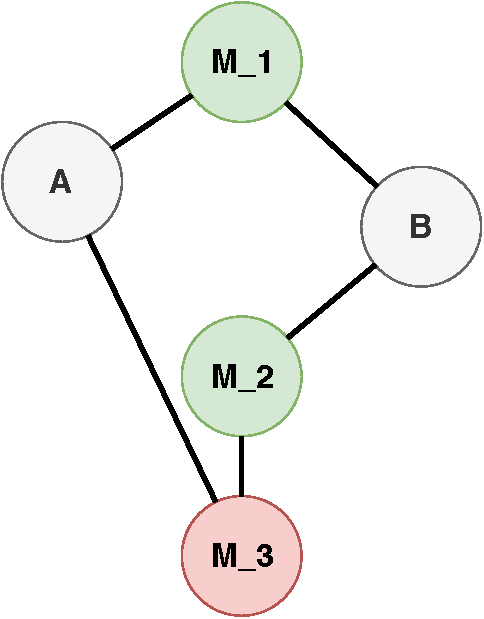
\includegraphics[width=40mm, keepaspectratio]{img/branch_conflict.pdf}
\caption{A fenti példa illusztrálva. Megfigyelhető miként hibásodik meg az alkalmazás.}
\end{figure}

Egy olyan megoldásra lenne szükségünk ami teszteli a főágon megjelenő kódot még mielőtt az ténylegesen odakerülne. Ezt nevezik \textit{Continuous Integration}nak: A CI rendszer automatikusan ellenőrzi a főágba kerülő kódot még az integráció tényleges megtörténte előtt.\cite{CI_Atlassian} Így elértük azt, hogy mindig egy olyan kódbázis álljon a fejlesztők rendelkezésére mely bizonyítottan működőképes. De ez még nem jelenti azt, hogy a felhasználók által aktuális használt verziónak megfelelő kódot fogják szerkeszteni. Ha megbízunk a tesztekben amiket alkalmazásunkhoz írunk, akkor használhatjuk a CI/CD másik felét, a \textit{Continuous Deploymentet}.
\subsubsection{Continuous Deployment}
Continuous Deployment alatt azt értjük, hogy emberi beavatkozás nélkül, automatikusan a felhasználók elé kerül a kész termék. Ennek egyik legnagyobb előnye, hogy a fejlesztők szinte mindig azt a kódbázist kapják melyből a felhasználó előtt szereplő program épült.\cite{CD_Atlassian}

Érdemes megemlíteni, hogy stratégiai döntés lehet az is, hogy nem kerül automatikusan a felhasználók elé a termék, ahhoz emberi beavatkozás kell. Ezt \textit{Continuous Delivery}nek nevezik. Itt gyakorlatilag egy bármelyik pillanatban "élesíthető", lefordított alkalmazás keletkezik, melynek telepítése emberi döntésen múlik.

Létezik köztes megoldás is mely személyes véleményem szerint a legideálisabb. Ha tehetjük akkor tartsunk fent egy - az éles rendszerrel ekvivalens - infrastruktúrát. Itt alkalmazzunk \textit{Continuous Deployment}et, míg az éles rendszeren csak \textit{Continuous Delivery}t: ha a tesztrendszeren valóban működik az alkalmazás, akkor kézzel telepíthetjük azt az éles infrastruktúrára is.
\subsection{Elasztikus skálázás}
Hibamentes alkalmazásunk nagyon megtetszett a felhasználóknak, és szembetaláljuk magunkat azzal a problémával, hogy túlterheltek a szerverek. Mit tehetünk? Több erőforrást adunk a kiszolgálónak, erősebb fizikai gépet, esetleg több példányt indítunk (több szerveren), és egy terheléselosztót illesztünk a program elé. Az elképzelés csodálatos, de van egy apró probléma: nem automatizált, emberi beavatkozás szükséges. Ez egyrészről probléma, mert valószínűleg nem tudjuk időben lekezelni a megnövekedett igényeket, nem tudunk időben felskálázni. Van azonban egy kevésbé nyilvánvaló ok is: költséghatékonyság szempontjából leskáláznunk is fontos, különösen ha felhőszolgáltatót\footnote{Távoli szervereket biztosító szolgáltató} használunk. Az éjjeli órákban egészen biztosan nem fog egy webalkalmazás akkora forgalmat generálni, mint mondjuk egy délután során.

Tehát a skálázás azt jelenti, hogy az alkalamazás számára rendelkezésre álló erőforrások mennyiségét szabályozni tudjuk. De mitől \textit{elasztikus}? Ez jelenti azt, hogy az igények alapján skálázunk. Nagy forgalom esetén fel, alacsony esetén le.\cite{Elastic_Turbonomic}
\section{A probléma fontossága}
A fentiek után azt gondolom nyilvánvaló miért (lenne) fontos minél több cégnek átgondolnia jelenlegi szoftverfejlesztési stratégiáját és élni a modern technológia adta lehetőségekkel. Verziókezelt kódot használni, tesztesetekkel, CI rendszerbe kötve és aztán automatikusan közzétéve, alkalmazástípustól függően skálázva azt.
\section{A tervezett megoldás}
Az eddig leírtak tükrében szeretném a példa webalkalmazás verziókezelését megvalósítani, mégpedig két kiemelt ággal:
\begin{itemize}
    \item \textit{prod} ág: A felhasználó elé kerülő verzió főága.
    \item \textit{beta} ág: Belső fejlesztéshez használt rendszer, teljesen különálló, de a \textit{prod} ággal megegyező infrastruktúrán (értelemszerűen kevesebb erőforrással).
\end{itemize}
Ezeket \textit{Continuous Integration} rendszer fogja védeni. Ide kódot olvasztani csak akkor lehet, ha a tesztek sikeresen lefutottak. Ha ezekre az ágakra új programkód érkezik, akkor ismét tesztelésre kerül, és ha sikerrel jár akkor alkalmazáskép\footnote{Olyan "fájl" mely alapján az alkalmazást el lehet indítani} készül, majd az a megfelelő infrastruktúrán telepítésre is kerül.

Az alkalmazás menedzselését, monitorozását, és a skálázást Kubernetes segítségével tervezem megvalósítani, melyről a továbbiak során szó fog esni.
\chapter{Az alkalmazás}
\section{Architektúrális felépítés}
A webshop program három fő résszel rendelkezik. Egy frontend, amit a felhasználó a böngészőből elér; egy backend, amivel a frontend kommunikál; ez pedig egy adatbázisból nyeri ki a termékek adatait. A frontend-backend kommunikáció HTTP-n keresztül történik, a chat funkcionalitás pedig WebSocket segítségével. A backend TCP kapcsolaton keresztül éri el az adatbázist.
\vskip 0.1in
\textit{Megjegyzés: az alkalmazás használt protokollokra a 2.1.3-as fejezetben részletesen kitérek.}
\begin{figure}[ht]
\centering
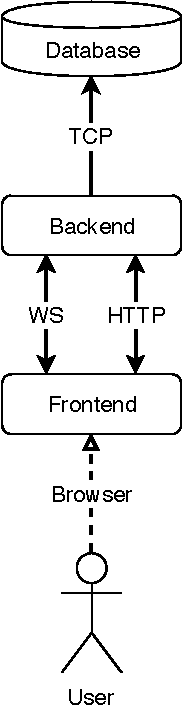
\includegraphics[width=24mm, keepaspectratio]{img/app_architecture.pdf}
\caption{A példa alkalmazás felépítése.}
\end{figure}
\vskip 0.1in
\newpage
\subsection{Frontend}
A webalkalmazás "látható" részét a frontend teszi ki. Reactban íródott ami egy JavaScript alapú web keretrendszer: a FaceBook hozta létre, és felhasználói felületek építésére használják.\cite{Node_W3} Mivel JavaScript alapú, így a programkód npm\footnote{Node Package Manager - \url{https://www.npmjs.com/}} segítségével fordítható.

A felület lehetőséget nyújt termékkategóriák böngészésére (ez a menüben dinamikusan generált), és ott termékek kosárba helyezésére. Továbbá chatelhetünk is az oldalon tartózkodó egyéb felhasználókkal.

\begin{figure}[ht]
\centering
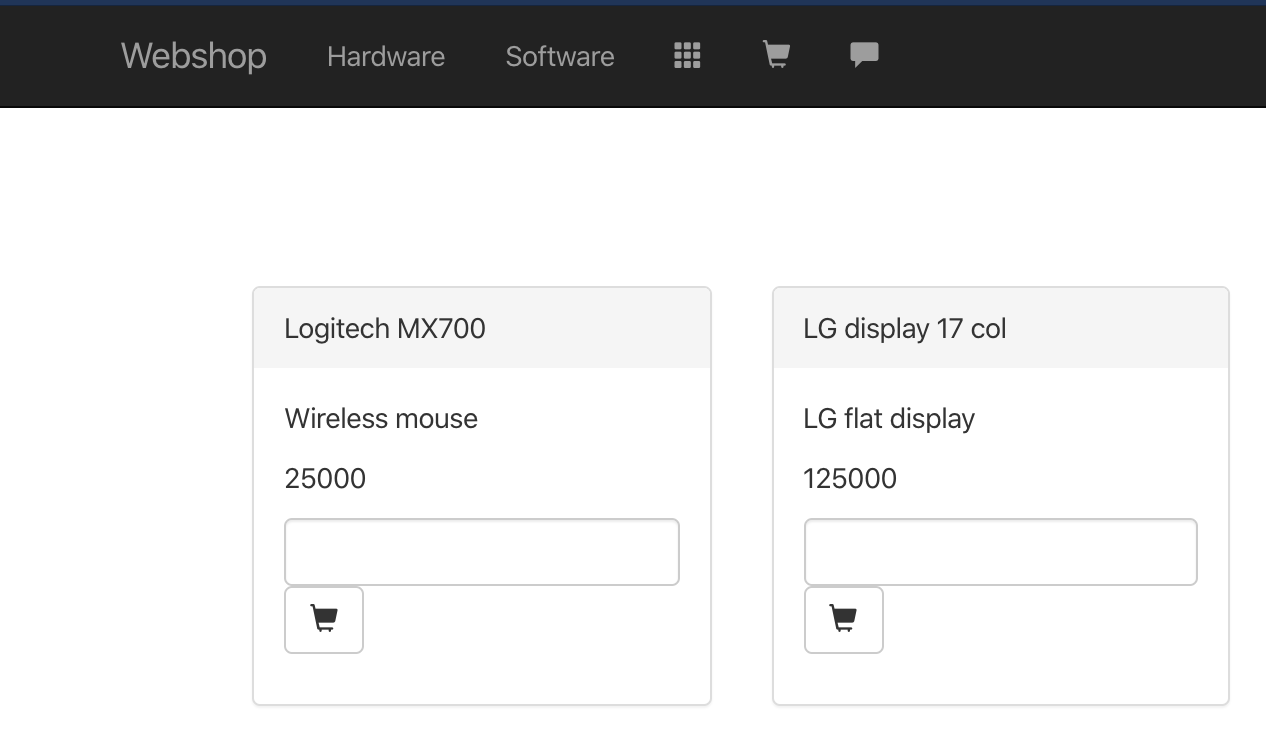
\includegraphics[width=150mm, keepaspectratio]{img/frontend.png}
\caption{Az alkalmazás kinézete.}
\end{figure}
\subsection{Backend}
A backend egy Springben íródott program. Ez egy Java alapú alkalmazás keretrendszer, mely 2003 óta létezik és jelenleg is aktív fejlesztés alatt ál. A futtathatóságot jelentősen leegyszerűsítendő, az alkalmazás Spring Boot-ot használ mely lényegében azt teszi lehetővé, hogy egy Springben írt alkalmazás \textit{click-to-run} (azaz egy kattintással futtatható) legyen.\cite{SpringBoot}

A program futtatáshoz le kell töltenünk a szükséges függőségeket és azt az alkalmazással együtt csomagolni. A backend készítői Maven buildkezelőt használnak, ami többek között a fenti feladatokat is ellátja.
\subsubsection{Adatbázis}
Az alkamazás a termékek listáját egy adatbázisból olvassa ki. Erre Postgres-t használ, egészen pontosan annak 11-es verzióját.
\vskip 0.1in
\textit{Megjegyzés: a használt adatbázismotor később lett Postgresre cserélve, mert a skálázás megvalósításához ez elkerülhetetlen volt. Eredetileg HyperSQL\footnote{Javaban írt adatbázismotor - \url{http://hsqldb.org/}} volt használva, azonban az a skálázáshoz létszükéges replikációt\footnote{Adatbázisok közti adatok szinkronizálása} nem támogatta.\cite{HSQL}}

Jelenleg két tábla létezik, az egyik a kategóriákat, míg a másik az azokba tartozó termékeket tárolja, ahogyan az az éles rendszerből lekért adatokon látszik:
\begin{lstlisting}
webshop=# \dt
          List of relations
 Schema |   Name   | Type  |  Owner
--------+----------+-------+----------
 public | category | table | postgres
 public | product  | table | postgres
(2 rows)

webshop=# select * from category;
 id |   name
----+----------
  1 | Hardware
  2 | Software
(2 rows)

webshop=# select * from product;
 id |          description           |          name           | price  | category_id
----+--------------------------------+-------------------------+--------+-------------
  1 | Wireless mouse                 | Logitech MX700          |  25000 |           1
  2 | LG flat display                | LG display 17 col       | 125000 |           1
  3 | Laser pointer and presenter    | Microsoft laser pointer |   6800 |           1
  4 | The best office suite for home | Ms Office 2018 Home     |  25000 |           2
  5 | Graphical editing software     | Adobe Photoshop         | 125000 |           2
(5 rows)
\end{lstlisting}
\subsection{Kommunikáció a rétegek közt}
Ahogyan az a 2.1-es ábrán látszik, három fő kommunikációs csatorna valósul meg a rétegek közt:
\begin{enumerate}
    \item Adatbázis <--> Backend: TCP\footnote{Transfer Control Protocol} segítségével történik az adatok lekérése. A backend JDBC Drivert\footnote{Java DataBase Connectivity API - Olyan Java komponens mely lehetővé teszi az adatbázissal való kommunikációt} használ, és a megalkotott SQL utasításokat elküldi az adatbázisnak, aki arra válaszul visszaküldi az eredményt.
    \item Backend <--> Frontend: HTTP segítéségvel, egy API végponthoz fordulva történik az adatok lekérése. Úgy kell elképzelni, hogy a frontend betöltésekor kapunk egy leírót, hogy hogyan néz ki az oldal, és hol van az adatok helye. De azoknak lekérése nem a frontend dolga, pusztán azt mondja meg hol találjuk azt. Ezek után a felhasználó böngészője már az backendhez fordul.
    \vskip 0.1in
    \textit{Megjegyzés: azért nem közvetlenül az adatbázishoz kapcsolódik a kliens mert ez nem biztonságos, például közvetlenül ki lehetne olvasni az adatbázistábla szerkezetét és akár olyan adatokat is, melyeket nem lenne szabad. A másik ok pedig, hogy így könnyen válthatunk adatbázismotort, hisz csak a backendet (sőt, ott is csak a JDBC drivert) kell cserélni.}
    \item Backend <--> Frontend: WebSocket segítségével zajlik a kommunikáció. Bár lentebb kifejtem részletesen, de röviden: a chat funkcionalitás megvalósítása miatt szükséges ezen protokoll bevezetése, hogy valós idejű kommunikáció jöhessen létre a szerver és kliens között.         
\end{enumerate}
\newpage
\subsubsection{HTTP}
\textbf{HyperText Transfer Protocol - a web alapja}

Bár a szakdolgozatom témájához szorosan nem kapcsolódik, mégis érdemesnek tartom ezt a féloldalas kitérőt a HTTP protokoll felé, hiszen a ma ismert web magjának részét képzi. Egy 24 éves alkalmazásbeli (\textit{7. rétegbeli}) protokollról beszélünk, mely a mai napig fejlesztés alatt áll: első verziója a HTTP/1.0 volt, (sajnos) jelenleg legelterjedtebb változata a HTTP/1.1\cite{ripHTTP2}, illetve 2015-ben jelent meg a modernnek számító HTTP/2.0\cite{HTTP2_RFC}

A könnyebb megértés érdekében szeretném részletezni a HTTP/1.1 protokollt.

Három alapvető részből épül fel:
\begin{itemize}
    \item \textbf{request line}
    \item \textbf{request body}
    \item \textbf{message body}
\end{itemize}
Talán a \textit{request line} a legfontosabb, mely két részből épül fel: egy kérés típusból illetve egy útvonalból melyhez a kérést intézzük. Az alábbi kéréstípusok léteznek:
\begin{itemize}
    \item \textbf{GET} - az erőforrás elérése, lekérdezése.
    \item \textbf{HEAD} - hasonló a GET metódushoz, azonban csak a fejlécet kérdezi le.
    \item \textbf{POST} - az elérni kívánt útvonaltól a \textit{message body}ban található adatok feldolgozását kérelmezi.
    \item \textbf{PUT} - hasonló a POST metódushoz, azonban feldolgozás helyett pusztán tárolást kér.
    \item \textbf{PATCH} - hasonló a PUT metódushoz, azonban ez csak a szolgáltatott adatokat írja felül, nem új bejegyzést hoz létre.
    \item \textbf{DELETE} - adatok törlését kérelmezi a kiszolgálótól.
    \item \textbf{TRACE} - a kiszolgáló válaszul a beérkezett HTTP kérést küldi vissza.
    \item \textbf{OPTIONS} - az elérhető HTTP metódusok lekérdezésére szolgál.
    \item \textbf{CONNECT} - TCP kapcsolat felépítésére ad lehetőséget.
\end{itemize}

A kiszolgáló válaszul szintén egy három részes csomagot küld.
\begin{itemize}
    \item \textbf{response status line}
    \item \textbf{response header}
    \item \textbf{message body}
\end{itemize}
Szintén az első részt szeretném részletezni, ugyanis hibakeresésekhez rendkívül hasznos. Ez három alrészből áll: HTTP verzió, HTTP státuszkód, rövid leírás a státusszal kapcsolatban. A státuszkódot az alábbi öt kategóriába lehet sorolni:
\begin{itemize}
    \item \textbf{1xx} - információ közlése
    \item \textbf{2xx} - sikeres művelet \textit{(Gyakorlati példa: HTTP200 - OK)}
    \item \textbf{3xx} - átirányítás
    \item \textbf{4xx} - kliensoldali hiba \textit{(Gyakorlati példa: HTTP404 - NOT FOUND)}
    \item \textbf{5xx} - szerveroldali hiba
\end{itemize}

\subsubsection{WebSocket}
A WebSocket protokoll kétirányú kommunikációt tesz lehetővé a kliens és a távoli kiszolgáló között. A kommunikáció megkezdése egy nyitó kézfogásból és egy egyszerű üzenetből áll, TCP felett. A protokoll célja, hogy a kliens és szerver közti kétirányú kommunikáció meg tudjon valósulni több HTTP kapcsolat létrehozása nélkül (ami egyébként RFC szerint sérti is a HTTP/1.1 szabányt\cite{HTTP_RFC})\cite{WS_RFC}.

Gyakori tévedés, hogy a WebSocket bármilyen formában is függ a HTTP protokolltól. Két megtévesztő tulajdonságot figyelhetünk meg ami erre okot adhat. Alapértelmezetten a WebSocket is 80-as porton kommunikál a HTTP-hez hasonlóan, illetve a TLS\footnote{Transport Layer Security} feletti, biztonságos változata is a 443-as porton (WebSocket Secure, HyperText Transfer Protocol Secure). A másik ok pedig az, hogy a kezdeti kézfogás egy HTTP Upgrade kérelemként jelenik meg a webkiszolgáló számára.
A WebSocket URI\footnote{Uniform Resource Identifier}-ja a következőképp néz ki:
\begin{itemize}
    \item Nem-biztonságos kapcsolat definiálása esetén: \lstinline{ws://}
    \item Biztonságos, TLS feletti kapcsolat kérése esetén: \lstinline{wss://}
\end{itemize}

\textbf{A példaalkalmazás természetesen biztonságos kapcsolatot fog használni mind WebSocket, mind HTTP kommunikációra.}
\section{A hagyományos megközelítés}
Ebben a fejezetben azt szeretném megmutatni, hogy milyen lenne az alkalmazás fejlesztése és üzemeletetése, ha nem használnánk azokat a technikákat, technológiákat amikről egyébként a dolgozatom szól.
\subsection{Fejlesztés}
Ahogy azt az 1.1.1.1-es fejezetben már bemutattam, \textit{Continuous Integration} nélkül nem gördülékeny a fejlesztés. A csapatoknak magasszintű kooperációra van szükségük, ezáltal értékes mérnökórák vesznének el a fejlesztők (vagy a csapaton belüli emberek) koordinálására. Tehát legjobb esetben is azt feltételezhetjük, hogy a fejlesztés során verziókezelt kódbázissal dolgoznak.
\subsubsection{Tesztelés}
A tesztelésnél sajnos már korántsem biztos, hogy élnék azzal a feltételezéssel, hogy egyáltalán van átfogó tesztelés a szoftverfejlesztés ciklusában. Tegyük fel, létezik ilyen, vannak a programhoz készült tesztesetek. Ekkor ezt célszerű lenne minden programkód-kiadás előtt lefuttatni. De ez ismételten az automatizálás hiányából eredő időkidobás lenne. 
\subsubsection{Alkalmazásfrissítés}
Tételezzük fel, hogy a tesztelt webalkalmazás összes szükséges eleme rendelkezésünkre áll. Rosszabb esetben egyszerre kellene három komponenst cserélnünk. Mivel nem automatizált a módszer így ez időt vehet igénybe (és ismét értékes mérnökórák vesznek el...), de még vállalható lenne, és webalkalmazás esetén minimális (de nem nulla idejű) kieséssel járna. Viszont tegyük fel, hogy az alkalmazásból több példány fut egyszerre. Ez már kezelhetetlen lenne, hatékonyabb megoldás szükséges.
\subsection{Üzemeltetés}
Egy ilyen webalkalmazás üzemeltetésére többféle infrastruktúrát / megoldást lehete alkalmazni, mindegyiknek van előnye és hátránya is. Több dologra érdemes figyelni: költséghatékonyság, üzembiztonság, karbantarthatóság.
\subsubsection{Infrastruktúrális áttekintés}
A legegyszerűbb megoldás: mindent egy szerverre telepíteni és készen is vagyunk. Egy számítógépet kell venni, valószínűleg egy ideig az erőforráskihasználtság is optimális szinten lesz, mégis talán ez a legrosszabb megoldás. Mi történik akkor ha az eszköz meghibásodik? Szolgáltatáskieséssel kell számolnunk, mégpedig nem is röviddel. Csinálhatjuk azt is, hogy több kiszolgálót veszünk és mindenki a maga feladatát látja el (egy kiszolgáló - egy alkalmazáskomponens). Ez talán mégrosszabb gondolat, mert háromszoros lesz a meghibásodás esélye. Valami olyan megoldás kellene ami magasabb rendelkezésreállást tud nyújtani. Csinálhatunk egy klasztert\footnote{Összefűzött számítógépek, melyek egységnek tekinthetőek}, tehát több gépre telepítjük fel az alkalmazás mindhárom komponensét és ezeket egy terheléselosztó (\textit{Load-Balancer}) mögé helyezzük, ezzel biztosítva azt, hogy egy kiszolgáló (vagy alkalmazás) meghibásodása esetén még szolgáltatni tudunk.

Egy költséghatékonyabb és izoláltabb (biztonságosabb) megoldást jelenthet a \textit{virtualizáció} alkalmazása, ahol a fizikai számítógépek gyakorlatilag virtualizált környezetben (számítógépeken) futtatnak operációs rendszert, amire aztán az alkalmazáskomponensek telepíthetőek. Így például változó erőforrásméretű gépeket is költséghatékonyan ki tudunk használni (értsd: mondjuk kétszer annyi komponens az "erősebb" kiszolgálón).
\chapter{Technológiai háttér}
A feladat megoldásához szükséges ismerni a rendelkezésünkre álló technológiákat és azokat több szempontból megvizsgálni:
\begin{itemize}
    \item A legfontosabb természetesen az, hogy az adott technológia egyáltalán képes e biztosítani a követelményekben foglaltakat.
    \item A következő az implementáció könnyedsége és hatékonysága. Nem mindegy, hogy az adott technológiával csak megoldani tudjuk a problémát, az is fontos, hogy az valóban "arra legyen kitalálva" amire használni szeretnénk.
    \item A harmadik szempont bizonyos esetben fontosságban az implementációs könnyebbség elé is kerülhet: a költséghatékonyság. Már a dolgozatom írása során is előkerült egy jelentős különbség két szolgáltató között, melyről részletesebben az 5.1.-es fejezetben írok.
\end{itemize}
\section{Felhőszolgáltatások}
Napjainban egyre népszerűbb és költséghatékonyabb az úgynevezett \textit{Cloud Computing} lehetőségével élni. Ennek lényege, hogy nem szükséges saját magunknak a fizikai eszközöket (pl.: szervereket) beszerezni, hanem bérelhetünk egy szolgáltatótól számítási kapacitást. Többféle modell létezik, ezek közül a három legnépszerűbbet szeretném bemutatni:
\begin{itemize}
    \item Infrastructure as a Service (IaaS) - gyakorlatilag ez megfeleltethető egy távoli infrastruktúrának amiről máskülönben nekünk kellene gondoskodnunk. Ezek különböző komponensekből állhatnak, úgymint szerverek, tárterület, hálózat.
    \item Platform as a Service (PaaS) - hasonló a \textit{IaaS}-hoz, de itt több alkalmazásbeli réteget biztosítanak, például az operációs rendszert sem kell menedzselnünk többé, csupán az általunk futtatni kívánt alkalmazást és annak adatait.
    \item Software as a Service (SaaS) - gyakorlatilag a programok felhőben futó változata. Több olyan szoftver létezik aminek van úgynevezett \textit{self-hosted} (magunknak kiszolgált) változata és a kiadó által biztosított is.
\end{itemize}
\begin{figure}[ht]
\centering
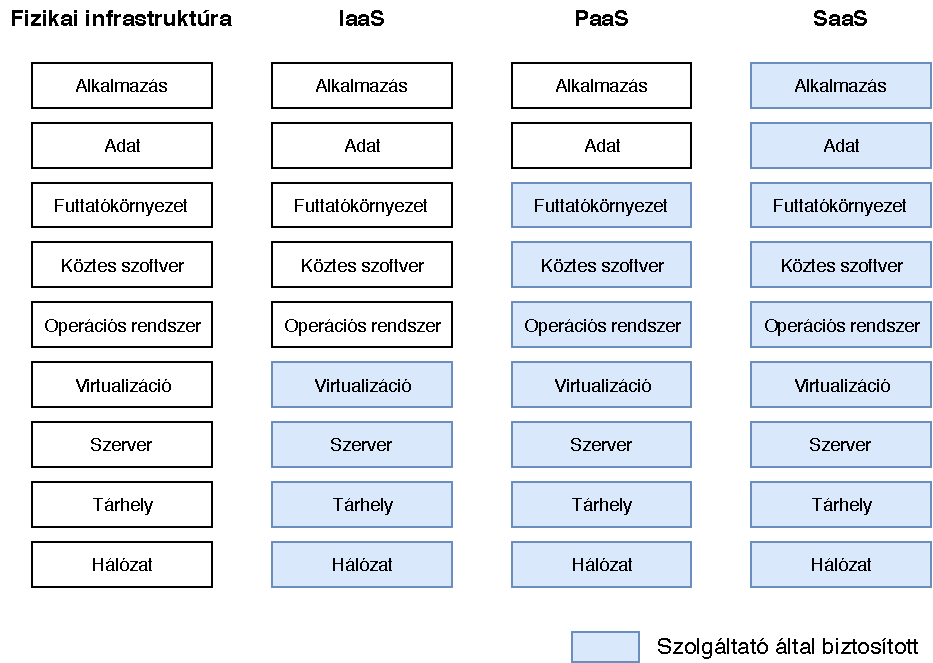
\includegraphics[width=150mm, keepaspectratio]{img/XaaS.pdf}
\caption{Különböző szolgáltatási modellek}
\end{figure}
\newpage
\vskip 0.1in
\subsection{Google Cloud Platform}
A Google 2008-ban indította útnak saját felhőszolgáltatását\footnote{\url{https://cloud.google.com/}}, ezzel komoly konkurenciát teremtve az Amazonnak aki akkor már két éve a piacon volt. Jelentős sikereket ért el, melyet legfőképp az infrastruktúra üzembiztonságának köszönhet, egy időben a marketing anyagokban is úgy fogalmaztak, hogy lehetőségünk van ugyanott futtatni alkalmazásainkat ahol a Google saját eszközei is megtalálhatóak.

Minden új felhasználónak lehetősége van igénybevenni 300 amerikai dollár kezdőegyenleget, mely szabadon felhasználható minden szolgáltatáshoz, illetve időnként promóciók keretében még többre is szert tehetünk (nemrég a GitLabbal szerződtek, így plusz 200 dollárhoz lehetett jutni). Nyújtanak továbbá oktatási támogatást is, azonban inkább projektekre és kutatásokra vonatkozik e kedvezmény, egy szakdolgozathoz én nem tudtam igénybevenni.

Szolgáltatási modellek terén megtalálható az \textit{Infrastructure as a Service}, ennek legfőbb terméke a \textit{Compute Engine}, ahol gyakorlatilag szervereket bérelhetünk általunk meghatározott operációs rendszerrel, és válaszhatunk többféle erőforrásmennyiség közül is. Érdekes megjegyezni, hogy válaszhatunk az adott feladathoz legjobban illő hardvert is, van például processzoroptimalizált és memóriaoptimalizált géptípus is. A \textit{Kubernetes Engine} a \textit{Platform as a Service} kategóriába sorolható és mint neve is mondja egy menedzselt Kubernetes klasztert ad számunkra, melyről később még szó fog esni. Ehhez kapcsolódik egy \textit{Software as a Service} szolgáltatás, mégpedig a \textit{Google Container Registry} ami egy konténerkép-tároló, melyről szintén szó fog esni, hogy pontosan mire szolgál. Természetesen több száz terméke létezik még a szolgáltatónak, de a dolgozatom megírása során közvetlenül ezzel a hárommal találkoztam.
\subsection{Amazon Web Services}
Az Amazon tulajdonában álló felhőszolgáltatás az ismertebbek közül a legrégebbi a piacon: az Amazon Web Services 2006 óta működik. Egyáltalán nem nevezhetjük olcsónak, azonban mivel az egyik legnagyobb tapasztalattal rendelkező cég, így sokan emiatt választják őket. 
\begin{figure}[ht]
\centering
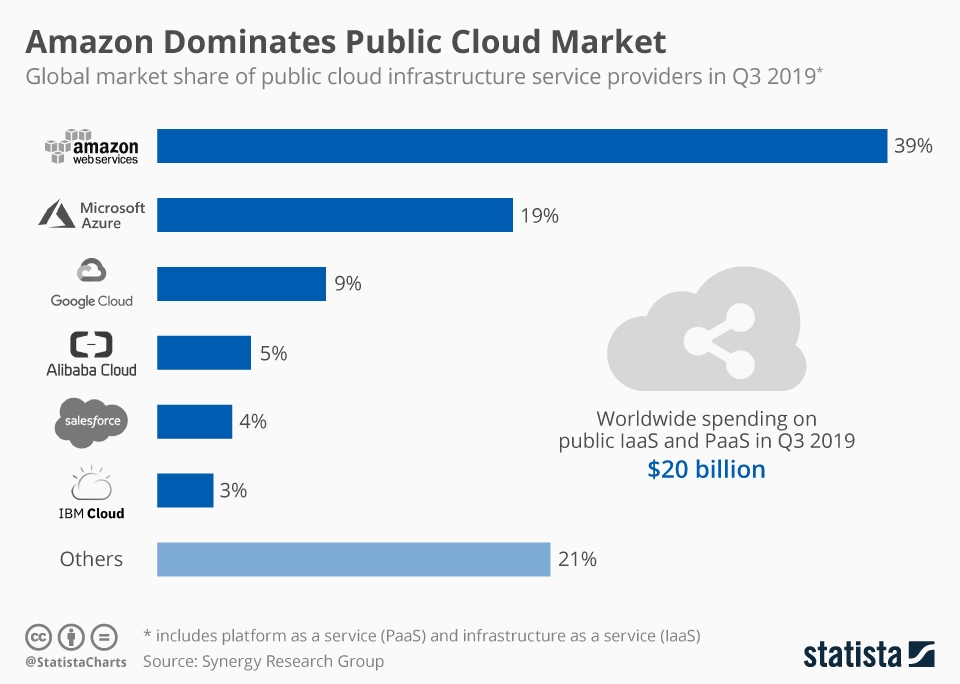
\includegraphics[width=150mm, keepaspectratio]{img/cloudproviders.jpg}
\caption{Felhőszolgáltatók piaci részesedése 2019-ben\cite{AWSshare}}
\end{figure}
\vskip 0.1in
Az új felhasználóknak úgynevezett \textit{free tier} (ingyenes szint) biztosított arra, hogy megismerje a terméket. Ezzel bár nem minden szolgáltatást lehet igénybevenni, de meg lehet ismerni mire képes a platform. Például ingyenesen lehet nagyon kis erőforráshasználatú szervert bérelni. Nyújtanak továbbá diákoknak havi 40 amerikai dollár támogatást, mely már több szolgáltatás használatára feljogosít. GitHub Student Developer Pack\footnote{\url{https://education.github.com/pack}} segítségével pedig további 110 dollárra tehetünk szert, mely már egész sok dolog kipróbálására elégséges.
\subsubsection{Elastic Compute Cloud (EC2)}
Az Amazon által nyújtott egyik legalapvetőbb \textit{Infrastructure as a Service} szolgáltatás, ahol rengeteg elődefiniált erőforráskombináció közül választhatjuk ki azt a géptípust amire nekünk szükségünk van. Természetesen ezen gépek az Amazon nagysebességű hálózatához csatlakoznak, és árkategóriától függően akár 10 Gbps sebességgel is tudnak a világhálón kommunikálni.
\subsubsection{Elastic Kubernetes Service (EKS)}
Az EKS egy menedzselt Kubernetes szolgáltatást biztosít mint \textit{Platform as a Service}. Fontos megjegyezni, hogy a worker számítógépekért (lásd: 3.4.1. fejezet) külön szükséges fizetni, hiszen azok gyakorlatilag előkonfigurált EC2 példányok. Az EKS egyébként sem mondható a legolcsóbb szolgáltatások közé, óránként 0.20 amerikai dollárt kell fizetnünk, és ez a workerek költségét nem is tartalmazza. Természetesen ez a havi 144\$ állandó összeg, tehát akár csak egy szolgáltatást futtatunk a klaszerben, akár ezret, ennyit fogunk fizetni a klaszter fenntartásáért.

A szolgáltatás nagymértékben integrálódik a lentebb felsorolt Amazon termékekkel, ezzel egy hatalmas előnyt állítva a saját kézzel összerakott Kubernetessel szemben.

\textit{Megjegyzés: az Amazonnak van egy saját - Kubernetes-szerű - szolgáltatása, az Elastic Container Service (ECS), mely lényegesen olcsóbb, nincs menedzsment költség, csak a workerekért kell fizetni.}
\subsubsection{Elastic Container Registry (ECR)}
Szintén egy későbbi fejezetben teszek említést a konténerekről, de röviden: alkalmazásainkat tárolhatjuk verziókezelt formában egy biztonságos, privát, és Kubernetes kompatibilis helyen. Előnye, hogy integrálódik az EKS-sel, illetve az Amazon jogosultságkezésével is (IAM).
\subsubsection{Virtual Private Cloud (VPC)}
Jogosan merül fel a kérdés, hogy például mi van akkor ha két kiszolgálót össze szeretnénk kötni hálózaton keresztül, de csak intraneten, helyi hálózaton. Hogy tehetjük meg ezt a felhőben? Sok egyéb mellett a VPC erre is alkalmas. Gyakorlatilag hálózatot építhetünk a felhőben.

A könnyebb áttekinthetőség érdekében tekintsük meg ezt az ábrát a hivatalos dokumentációból\cite{VPC}:
\newpage
\begin{figure}[!ht]
\centering
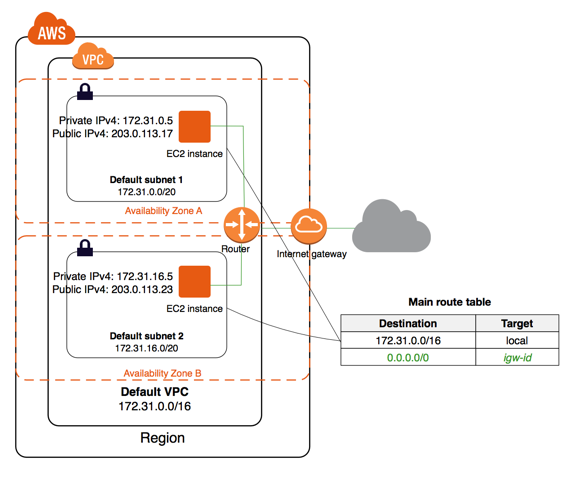
\includegraphics[width=150mm, keepaspectratio]{img/VPC.png}
\caption{A VPC működése}
\end{figure}
\vskip 0.1in
Az ábrán két kiszolgálót futtatunk (\textit{EC2 instance}), két külön elérhetőségi zónában (ezt azt jelenti, hogy bár egy régióban található a két adatközpont, azok izoláltak egymáshoz képest és egy alacsony késleltetésű kapcsolattal vannak összekötve). Mindkét kiszolgálónak van publikus és privát IP-címe is. Az elérhetőségi zónák között belső router irányítja a forgalmat, így az a publikus internet felé soha nem megy ki. A szándékosan külvilág felé/felől érkező csomagokat pedig az internet átjáró kezeli, mely szintén a routert használja.

Természetesen számos konfigurációs lehetőség van, például lehet ACL\footnote{Access Control List - kommunikáció/hozzáférés szabályozása}-eket beállítani. Az AWS alapértelmezetten konfigurál egy VPCt az EC2 példányoknak, és a szakdolgozatom kidolgozásához ez teljesen megfelelőnek bizonyult, így részletesebben nem térek ki a további lehetőségekre, azonban az alapvető működés megértését fontosnak gondolom.
\subsubsection{Elastic Load Balancing (ELB)}
Az Amazon terheléselosztója képes egy vagy több elérhetőségi zónán belül automatikusan elosztani az alkalmazások felé tartó forgalmat, legyen az EC2 példány, vagy egyéb szolgáltatások. Alapvetően kétféle terheléselosztót használhatunk, melyek mindegyike támogat olyan szolgáltatásokat mint a magas rendelkezésre állás, automatikus skálázódás illetve a beépített biztonsági funkciók:
\begin{itemize}
    \item Alkalmazásszintű terheléselosztó (\textit{Application Load Balancer}) - Leginkább HTTP és HTTPS forgalom elosztására tervezték, az OSI réteg\footnote{Open Systems Interconnection Reference Model, összesen hét szint} hetedik szintjén\footnote{Alkalmazásréteg} működik, és az Amazon VPC felé irányítja a kéréseket, azok tartalma alapján.
    \item Hálózati szintű terheléselosztó (\textit{Network Load Balancer}) - Leginkább TCP és UDP\footnote{User Datagram Protocol} forgalom elosztására tervezték, az OSI réteg negyedik szintjén\footnote{Szállítási réteg} működik, és az Amazon VPC felé irányítja a kéréseket, akár több milliót másodpercenként.
\end{itemize}
\subsubsection{Identity and Access Management (IAM)}
Egy hatalmas infrastruktúrához robosztus jogosultságkezelésre van szükség, és az Amazon IAM pontosan ezt valósítja meg. A szolgáltatás segítségével létrehozhatunk és menedzselhetünk AWS felhasználókat, csoportokat és jogosultságokat adhatunk nekik egy adott erőforrás elérésének engedélyezésére vagy megtagadására. Ha újrafelhasználni is szeretnénk egy adott engedélycsoportot akkor \textit{szerepbe} érdemes csoportosítani őket. A szerep engedélyek összessége és így egyszerűbben lehet adott személyhez, szolgáltatáshoz, vagy csoporthoz rendelni azt. Továbbá: ezeket a szerepeket meg lehet személyesíteni és fel lehet venni. Ezt azt jelenti, hogy nem kell mindenféleképp állandóan bírni egy adott jogosultsággal, csak amikor az ténylegesen indokolt. Például veszélyes lehet a napi munka során egy olyan jogkörrel bírni ami minden erőforrás törlésére jogosult, azonban néha előfordulhat hogy erre szükség van.
\section{Microservice architektúra}
Régen az emberek monolit alkalmazásokat írtak. Az ilyen típusú alkalmazások funkciói egyetlen kódbázisban, azaz egyetlen hatalmas programban valósulnak meg. Ez a fejlesztési fázis elején, kis projekteknél kényelmes, azonban hosszabbtávon nem kifizetődő.
\begin{figure}[!ht]
\centering
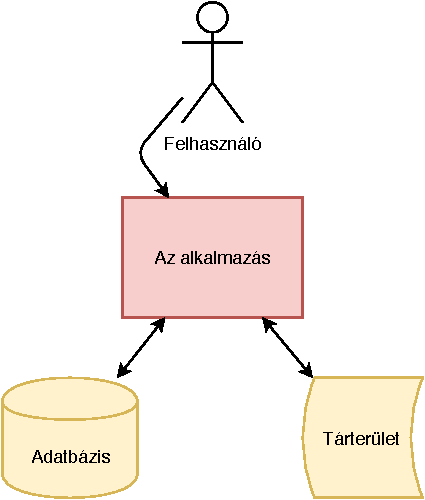
\includegraphics[width=60mm, keepaspectratio]{img/app_monolit.pdf}
\caption{A monolit alkalmazás felépítése}
\end{figure}
\vskip 0.1in
Mi is a probléma ezekkel a hatalmas alkalmazásokkal? Nagyobb terhelés mellett az egész szolgáltatás összeomolhat, még akkor is ha szorosan nem függnek egymástól az adott funkciók. Nehezen skálázható, csupán egy adott kiszolgálón futhat, nem lehet a részeit "szétszedni" és külön hardverre helyezni. A közös kódbázisból pedig a nehezebb fejleszthetőség problémája ered, hiszen mindenki ugyanazon forráskódot, továbbá elképzelhető, hogy az funkciók felelősei sincsenek teljesen pontosan meghatározva. (Például, hogy direkt vagy indirekt módon egy olyan osztálytól függ egy másik, melyről nem is gondolnánk).
\vskip 0.1in
A fenti leírásban már sugalltam, hogy mi a felsorolt problémákra a megoldás: találnunk kell egy módot, hogy valahogy izoláljuk alkalmazásunk egyes részeit, praktikusan funkcionalitás alapján.
\begin{figure}[!ht]
\centering
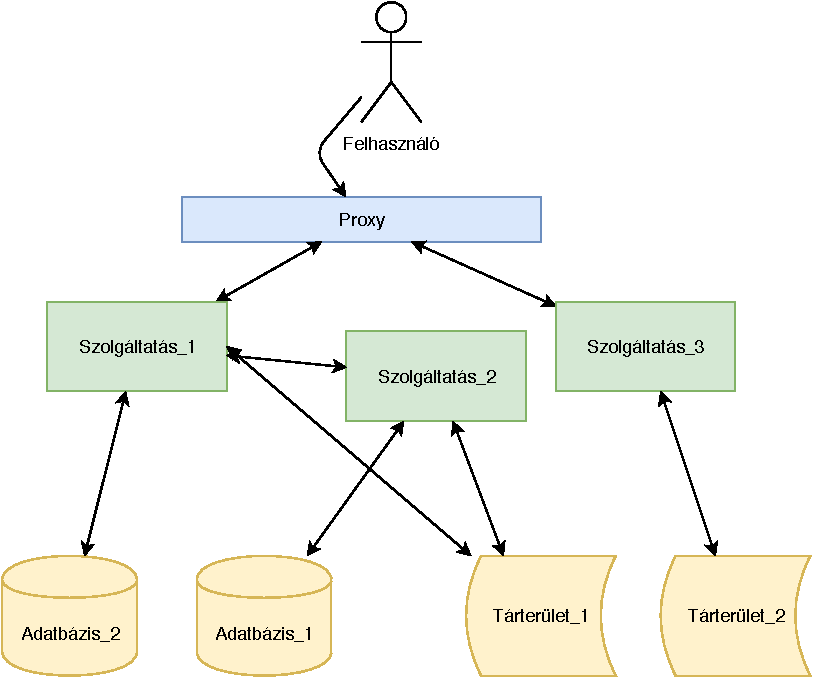
\includegraphics[width=125mm, keepaspectratio]{img/app_micro.pdf}
\caption{Egy egyszerűbb szolgáltatás, három mikroszolgáltatással megvalósítva}
\end{figure}
\vskip 0.1in
Az alkalmazásunk kódja is szeparált lett, könnyebb fejlesztőcsapatokat egy adott szolgáltatáshoz rendelni, továbbá a skálázhatóság is egyszerűbb, hiszen már akár több kiszolgálóra és elhelyezhetjük a különböző komponenseket. Ez utóbbit \textit{horizontális skálázás}nak nevezzük, míg mikor egy adott kiszolgálót bővítünk azt \textit{vertikális skálázásnak}.
\subsection{Stateful és stateless alkalmazások}
Tegyük fel, hogy hiába bontottuk szét alkalmazásunkat, az egyik mikroszolgáltatás olyan szintű terhelést kap, ami még egy dedikált kiszolgáló (tehát csak ezt az egy szolgáltatást futtatjuk) számára is kezelhetetlenül sok. Felmerülhet bennünk az ötlet, hogy indítsük el több példányban ezt a szolgáltatást és alkalmazzunk terheléselosztást a kettő között. Például egy fizetést megvalósító szolgáltatás ami egy \textit{Payment Gateway}\footnote{fizetési szolgáltatást biztosító "kapu"}-el kommunikál az ilymód skálázható, azonban ha mondjuk szeretnénk eltárolni azon felhasználók adatait akik fizettek, akkor ezen adatbázis nem. Miért? Mert a Payment Gateway API állapotmentes, nincs olyan amit tartósan tárolni kellene így mindegy melyik szolgáltatáshoz irányít minket a terheléselosztó. Egy adatbázisnak viszont pont a tárolás a lényege, így tulajdonképpen attól függene a visszaadott adathalmaz, hogy melyik példányhoz lettünk irányítva.

Előbbi szolgáltatást állapotmentesnek (\textit{statelessnek}, utóbbit pedig állapottól függőnek (\textit{statefulnak}) nevezünk. A stateful alkalmazások nehezen (vagy nem) skálázhatóak.
\section{Konténerizáció}
Régóta problémát jelentett, hogy egy adott alkalmazásnak számos függősége lehet, például hogy egy adott könyvtár/szoftver meglétére volt szükség hogy a programkód egyáltalán leforduljon. Ebből eredtek azok a problémák, hogy ami a fejlesztő gépén még futott az máshol már nem biztosan. Legnagyobb problémának viszont a függőségek úgynevezett ütközései bizonyoltak: tételezzük fel, hogy egyik alkalmazásunk \textbf{K könyvtár} 1.1-es verzióját szeretné használni, míg egy másik \textbf{K könyvtár} 2.0-s verzióját. Jobb esetben elfogadja az új a régit, de ez nem mindig ilyen egyszerű.

Erre a problémára is (és rengeteg, ennél fontosabbra is) megoldást találtak, mégpedig a \textit{virtualizáció}t. Ez a technológia lehetővé teszi egy fizikai kiszolgálón több logikai számítógép létrehozását a hardverelemek virtualizálásval. Ez azt jelenti, hogy a fizikai gépre (\textit{gazda}) telepítenünk kell egy \textit{hypervisor}t, mely az erőforrások elosztásáért és emulálásáért felelős. Ezek után a virtuális gépekre (\textit{vendég}) telepíteni kell operációs rendszert, és arra az alkalmazást. Hatékony technológia, és jelentősen megkönnyíti az erőforrások elosztását, költséghatékony megoldást teremtve.

Egy ideje azonban már a konténerizáció is jelen van, mely bizonyos tekintetben (természetesen több limitációval) hasonlít a virtualizációra és kevesebb erőforrást emészt fel a gazdagéptől. Az egyszerűbb megértés végett tekintsük meg ezt az ábrát:
\begin{figure}[ht]
\centering
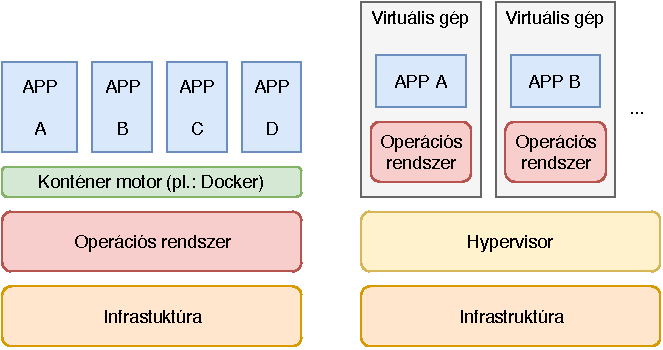
\includegraphics[width=125mm, keepaspectratio]{img/virtcont.pdf}
\caption{Konténerizáció és virtualizáció}
\end{figure}
\vskip 0.1in
Érdemes megfigyelni, hogy nincs többé szükségünk több operációs rendszer telepítésére, mely például egy Windows telepítés esetén súlyos "felesleges" erőforrást emésztene fel. Az ilymód futtatott alkalmazások a lehető legnagyobb mértékben izoláltan futnak, de egy közös operációs rendszeren, annak a szintjén szétválasztva. Több megoldás is létezik, például LXC, Jails vagy éppen a Docker.
\subsection{Docker}
A Docker 2013-ban látott napvilágot, azonban a kezdeti verziók meglehetősen instabilnak bizonyoltak. Ez az operációs rendszer szintű virtualizáció a Linux kernel számos képességét használja ki, mint például a névterek, a Netfilter vagy a cgroupok. A termék sikerességét bizonyítja, hogy a termék már MacOS-en és Windows rendszeren is használható.
A konténereket (amik gyakorlatilag a futtatható alkalmazások és függőségeik) \textit{kép}ekben tároljuk. Ha ilyen képet szeretnénk készíteni akkor úgynevezett \textit{Dockerfile}-t kell írnunk. A megadott utasítások alapján a Docker elvégzi a feladatot és utána a konténerkép segítségével konténerpéldányokat lehet indítnai.

Egy példa Dockerfile:
\begin{lstlisting}
FROM ubuntu:18.04      # az ubuntu konténerképből induluk ki, a 18.04es verzióból
COPY . /app            # a jelenlegi mappából a konténer /app mappájába másoljuk a fájlokat
RUN make /app          # a kép építése során végrehajtjuk a make /app parancsot
CMD python /app/app.py # a konténerkép futtatásakor az alábbi parancs fog végrehajtódni
\end{lstlisting}
\subsubsection{Registryk}
A Dockerfileban láttuk, hogy egy ubuntu képre hivatkozunk. De honnan van nekünk meg ez a kép? Nincsen. Egy Docker Hub nevű \textit{registry}ben tárolódik. A registryre úgy kell tekinteni mint egy konténerkép tároló. Ráadásul egyazon konténerből többféle verziót is közzétehetünk, ezt szolgálják a \textit{tag}ek melyet kettőspont után lehet írni (a fenti példában 18.04). Képet letölteni a \lstinline{pull}, feltölteni a helyi képek közül pedig a \lstinline{push} paranccsal lehet.

Létezek privát registryk is, hiszen nem mindenki szeretné az alkalamazását közzétenni az egész világ számára. Bár a Docker Hub is nyújt erre lehetőséget, ingyenesen csak egy repositorynk lehet, utána viszont fizetnünk kell, mégpedig nem keveset. Költséghatékonyabb megoldás például az \textit{Amazon Container Registryt (ECR)} használni, mely alapértelmezetten privát.
\section{Konténer orkesztráció}
Egy modern alkalmazás több száz mikroszolgáltatásból is állhat, melyek laza kötésű konténerekként jelennek meg. Konténer orkesztráció alatt ezen konténerek együttműködésének megszervezését jelentjük.\cite{ContOrch}

Több rendelkezésünkre álló technológia közül válaszhatunk, ilyen például az \textit{Apache Mesos}, \textit{Docker Swarm} és a \textit{Kubernetes}. Ezek mindegyike saját módszer alapján biztosítja a konténerek felügyeletetét, azok életciklusának kezelését, egészségüknek monitorozását, skálázását és frissítését.
\subsection{Kubernetes}
A Kubernetes 2014 nyarán jelent meg a Google gondozásában, és egy Dockerre épülő konténer orkesztrációs platformot valósít meg. Gyakran "k8s" néven is emlegetik.
\subsubsection{Alapfogalmak}
A Kubernetes alapvető működését objektumok határozzák meg, melyekből a fontosabbakat pár mondatban összefoglalom\cite{k8s}:
\begin{itemize}
    \item \textbf{Namespace} - A névterek egyfajta izolációs célt szolgálnak, gyakorlatilag egy virtuális klaszter a klaszterben.
    \item \textbf{Pod} - A Kubernetes legkisebb egysége. Konténerek összessége és az azokhoz tartozó alapvető konfigurációs beállítások mint például az igényelt erőforrások mennyisége.
    \item \textbf{Deployment} - A Deploymentek a Podok kezelésére szolgálnak. Megvalósíthatóak velük magas rendelkezésreállású szolgáltatások (több pod egyidejű futtatása), verziókezelés, skálázás.
    \item \textbf{Service} - Egy absztrakciós réteget von a Podok/Deployment hálózatkezelése felé. Megvalósít klaszteren belüli DNS bejegyzést és egy deployment alá tartozó podok felé érkező kommunikáció menedzselését.
    \item \textbf{Ingress} - A külvilágtól érkező kommunikációért felelős. Az adott Service HTTP és HTTPS útvonalait szolgálja ki, megadott szabályok alapján. Fontos, hogy az Ingress működéséhez egy úgynevezett Ingress Controllert kell telepíteni a klaszterbe, mely effektíve a forgalomirányítást végzi.
    \item \textbf{StatefulSet} - Az állapotfüggő szolgáltatások menedzselését hivatott elvégezni. Míg a deploymentnél teljesen lényegtelen például az indítási sorrend, addig egy stateful alkalmazásnál előfordulhat hogy ez igenis fontos.
    \item \textbf{ConfigMap} - Podok (és a bennük lévő konténerek) konfigurálására szolgál olymód, hogy azt nem közvetlen annak leíró fájlábab végezzük el, ezzel növelve az adott alkalmazás horozhatóságát. Fontos megjegyezni, hogy az érzékeny információk tárolására nem alkalmas, arra a \textit{Secret} objektum szolgál.
\end{itemize}
Ezeket az entitásokat úgynevezett \textit{.yaml} fájlban tudjuk leírni, ebből a negyedik fejezetben majd láthatunk párat.
\subsubsection{Magas rendelkezésre állás}
A Kubernetes segítségével szinte plusz befektetett energia nélkül tehetjük szolgáltatásunkat hibatűrővé. Egy Deployment létrehozásával és megfelelő konfigurálásával szinte azonnal elérhetjük célunkat. Frissítéskor úgynevezett \textit{Rolling Update} megy végbe: alapbeállítás szerint elindít egy podot, majd leállít egy régit. Ezt addig ismétli míg meghatározott számú pod nem lesz kész állapotban. Egy ilyen frissítésnél (és egyébként is) fontos megadni a Kubernetesnek, hogy hogyan tudja ellenőrizni hogy az alkalmazás elindult, illetve hogy nem hibásodott meg. Erre szolgál a \textit{ReadinessProbe} és a \textit{LivenessProbe}. Előbbi indításkor ellenőrzi mikor lesz kész a pod, utóbbi pedig már működés közben monitorozza azt. Ezek az ellenőrzések lehetnek egyszerű HTTP kérések, TCP ellenőrzés vagy egyéni alkalmazás futtatása konténeren belül.
\subsubsection{Terheléselosztás}
A Kubernetes a Service és az Ingress segítségével automatikusan elosztja az összetartozó podok közt a terhelést, így akár több állapotmentes alkalmazás tud ugyanazon feladat kisebb részeivel dolgozni.
\subsubsection{Skálázás}
A Kubernetes több szempont alapján és több módon teszi lehetővé a skálázást. Egyik legalapvetőbb módja a Deploymentben definiálni egy minimum és maximum podszám értéket, illetve hogy egy podnak milyen terhelést kell átlagosan kapnia hogy a skálázás végbemenjen.
\section{Verziókezelés}
Bár már többször említettem a verziókezelést dióhéjban, illetve annak fontosságát, a működését még nem írtam le. A lényeg alapvetően a változtatások követése, ezek verziózása és a lehetőség adott verzióra visszaállásra. Több megoldás létezik melyek implementációja eltér. Én most csak a Gitre fogok kitérni mivel az alkalmazás azt használja, de érdemes megemlíteni a \textit{Subversiont}, \textit{Mercurialt} és a \textit{Microsoft Team Foundation Servert} is.
\subsection{Git}
A Git szoftvert eredetileg Linus Torvalds fejlesztette ki a szintén általa írt Linux kernel forráskódjának kezelésére. Egyik legnagyobb újítása az volt, hogy nem kellett folyamatos kapcsolat egy központi szerverrel, hanem csak akkor kellett azt használni amikor szükség volt rá.

Megemlítek pár parancsot és azon keresztül adok egy alapvető képet a rendszer működéséről:
\begin{itemize}
    \item \textbf{commit} - Az elvégzett módosításokat egy új verzióba közzéteszi (de nem tölti fel a szerverre!)
    \item \textbf{push} - A repository lokális állapotát feltölti a szerverre.
    \item \textbf{clone} - Egy távoli szerveren lévő repositoryt tölt le a saját gépünkre.
    \item \textbf{pull} - A távoli szerveren lévő repository állapotát letölti és frissíti vele a lokálisat.
    \item \textbf{merge} - A paraméterül adott ágat az éppen aktuális ágba olvasztja.
    \item \textbf{rebase} - A paraméterül kapott ág commitjait alkalmazza az aktuális ágra.
    \item \textbf{revert} - Az adott commitra visszaállítja a repositoryt.
\end{itemize}
\subsection{GitHub}
A GitHub egy 2008-ban létrejött szolgáltatás, jelenleg a Microsoft tulajdonában. Megtalálható benne a Git összes "szerver" funkcionalitása és számos egyéb hozzáadott funkció is, például: hozzáférés-vezérlés, programhibák nyomonkövetése, wikicikkek írásának lehetősége, és rövid ideje már CI/CD funkcionalitást is találunk benne.

A szakdolgozatom szempontjából két fontos részt szeretnék kiemelni. Az egyik a pull requestek. Ezek több célt szolgálnak. Elsődleges funkcionalitása a főágra való beolvasztás áttekinthetőbbé tétele, illetve a közvetlenül főágra történő feltöltés tiltása. Publikus projekteknél például a közreműködés legszebb módja, ha letöltjük a kódot, egy külön ágon javítjuk a kódot, majd feltöltjük és pull requestet nyitunk. A másik fontos dolog, hogy a pull requestek arra is alkalmasak, hogy ezeken teszteket végezzünk, és csak akkor engedjük főágra a kódot ha ez sikeres volt. Többek között a fenti két szabály is megtalálható az úgynevezett \textit{Branch Protection Rules} között, mely a GitHub online felületén konfigurálható.
\section{CI/CD}
Ahogyan azt az 1.1.1.-es fejezetben kifejtettem, a \textit{Continuous Integration} és \textit{Continuous Deployment} rendkívül hasznos dolog, és értékes mérnökórákat lehet megtakarítani egy jól kidolgozott folyamat során, ugyanis se a projektek közti koordinációra, se az esetleges (CI hiányából fakadó) alkalmazáshibákra nem kell időt fordítani.

Jelenleg több szolgáltató is van aki különféle megoldásokat kínál. Talán az egyik legnépszerűbb a GitHubhoz használható \textit{Travis CI}, de már maguk a kódot tároló szolgáltatók is előálltak megoldásokkal. A \textit{GitLabon} hosszú ideje létezik erre megoldás, a GitHub pedig az utóbbi fél év óta szintén kínál hasonló szolgáltatást\cite{GHAction}. Azonban én a szakdolgozatom során egy - mondhatni - ipari sztendertet fogok használni, a Jenkinst.
\subsection{Jenkins}
A szoftver 2005-ben került először piacra, akkor még \textit{Hudson} néven, a Sun Microsystemstől. 2011-ben nevezték át Jenkinsre (egészen pontosan leágaztatták). Sikerét konfigurálhatóságának és testreszabhatóságának köszönheti. Több száz bővítmény érhető el hozzá, és a folyamatokat Groovy nyelven is leírhatjuk.

Az alkalmazás alapvetően egy mesterből áll, és ezekhez lehet dolgozókat csatolni a teljesítmény növelése céljából. A mestert szintén be lehet állítani, hogy részt vegyen a munkában is.
\section{Monitorozás}
Egy szolgáltatásnak sem szabadna léteznie megfelelő monitorozás nélkül. Sajnos eddigi tapasztalataim alapján ezt sokan nem így látják és nem fektetnek ebbe energiát. Monitorozás alatt azt értem, hogy a szolgáltatást és/vagy az azt futtató infrastruktúrát valamilyen módon megfigyeljük (természetesen célszoftverekkel) és rendellenesség esetén súlyosságtól függően tájékoztatjuk az illetékes személyt a megfelelő csatornák igénybevételével.

Több szoftver is elérhető, régen a Zabbix volt a sztendert, de mára idejétmúltnak mondhatjuk. Ez a megoldás agentek telepítését követelte meg a monitorozni kívánt entitásra, és a metrikák úgynevezett \textit{push} módon érkeztek meg a Zabbix szerverhez ahol aztán azok feldolgozásra kerültek. Manapság inkább a Prometheus által kínált megoldást használják.
\subsection{Prometheus}
2014-ben kezdődött el a szoftver fejlesztése, Go programozási nyelvben. Ez azért érdekes mert minden komponens egy-egy binárisnak felel meg, nem szükséges telepítés. A Prometheus újdonságát az adja, hogy \textit{pull} módszerrel szerzi be a metrikákat: úgynevezett \textit{exporter}eket lehet telepíteni a monitorozandó entitásra \textit{vagy} egyéb helyre is. Ez a Go bináris egy apró webszerver segítségével teszi közzé az adatokat, amit a Prometheus konfigurálható időközönként beolvas és értelmez. Ezt nevezik \textit{scrape} műveletnek.

Természetesen az adatok gyűjtése még nem minősül monitorozásnak, arról riasztást is kell kapnia az érintetteknek. A Prometheushoz külön binárisban letölthető az \textit{AlertManager}, mely csoportosítja, deduplikálja a riasztásokat majd elküldi azokat, illetve figyeli ha egy aktív riasztás megoldódik. Természetesen karbantartási ablakokat is meg lehet határozni.
\subsection{Grafana}
Egy beérkező riasztás leírása nem minden esetben elég beszédes ahhoz, hogy meg tudjuk határozni pontosan hol van a hiba a rendszerben. Szükséges valamilyen vizualizációs eszköz is, erre pedig a tökéletes megoldás a Grafana nevű eszköz.
\begin{figure}[ht]
\centering
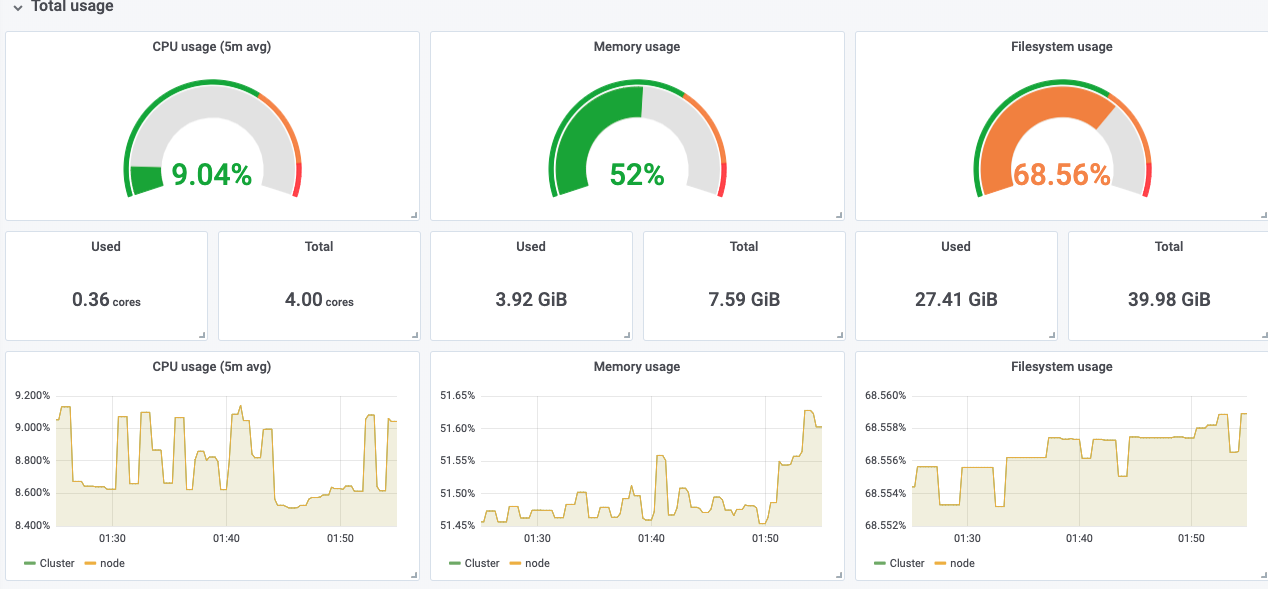
\includegraphics[width=150mm, keepaspectratio]{img/grafanaui.png}
\caption{A Grafana felhasználói felülete}
\end{figure}
\vskip 0.1in
A felületen különböző nézetek (\textit{dashboardok}) közül lehet választani, és ezeken \textit{Panel}ek jelenítik meg az adatot. Az adatok lekérdezésének a nyelve Prometheus adatforrás esetén \textit{PromQL}. Bár a Grafana felületén is lehetőség van riasztások létrehozására, személyes tapasztalatom alapján ez messze nem éri el az AlertManager (vagy hasonló technológiák) szintjét.
\chapter{Implementáció}
\textbf{Megjegyzés: a leírt lépések során feltételezem, hogy a számítógépen telepítve van \textit{docker} (kliens és motor egyaránt), illetve \textit{kubectl}\footnote{Kubernetes menedzsment eszköz} és \textit{awscli}\footnote{AWS parancssori alkalmazás}.}
\vskip 0.1in
Az előzetes tervezésem eredményeképp megállapítottam hogy mire lesz szükségem. Tudtam, hogy a Kubernetes lesz a fő "összetevő" hiszen a skálázás és a szolgáltatás alapvető monitorozása könnyen megvalósítható benne. CI/CD vonatkozásában több lehetőségem is volt, de a konzulensemmel történt egyeztetés alapján a Jenkinsre esett a választás. Noha külön virtuális gépre is helyezhettem volna, én a praktikusság kedvéért mindent egy klaszterre szerettem volna telepíteni, és ez így is történt. További alapvető teendőim voltak (bár ez a feladatkiírásban nem szerepelt) a klaszterszintű monitorozás megvalósítása. Ezt Prometheus és Grafana segítségével szerettem volna megvalósítani, melybe később a szolgáltatások is beköthetőek lehetnek.
\section{Alkalmazás Docker konténerekbe helyezése}
A Kubernetes Dockerre épül és az alkalmazások "telepítése" is konténerképek formájában történik, így hát legelső lépésben az alkalmazáskomponenseket kellett konténerizálnom, szerencsére az már funkcionalitás szerint frontendre és backendre volt bontva.

Azt hamar eldöntöttem, hogy a programkód fordítását és futtatását is Dockerben szeretném végezni, így éltem az úgynevezett \textit{Multi-stage build}\cite{multistage_docker} adta lehetőséggel miszerint több konténert is felhasználhatunk egy adott konténerkép előállításához. Ekkor ez utolsó konténerkép "rész" lesz az amit a konténer indításakor végrehajtunk. Esetemben kell egy konténer amiben a fordítás (\textit{build}) zajlik és egy másik ami a futtatókörnyezet. A fordítás az egyszerűbb művelet, legalábbis konténerizáció szempontjából. Az én esetemben a frontendet \textit{npm} programmal kellett fordítani, melyre kész konténer áll rendelkezésre \textit{node} néven. Ebbe a konténerbe kell másolni a forráskódot, majd a megfelelő parancsot kiadni. A backend esetén hasonló a lépés, ott a \textit{maven} konténerből érdemes kiindulni.

Előálltak a futtatandó alkalmazáskomponensek, azonban azoknak is meg kell határozni a futtatókörnyezetet: a frontend esetén erre a \textit{serve} csomagot alkalmaztam ami az npm csomagkezelővel letölthető, így itt is a \textit{node} konténerképből indultam ki. A backend esetében a fordítás produktuma egy darab \lstinline{.jar} fájl amihez Java 11 futtatókörnyezet volt szükséges: az \lstinline{openjdk:11} konténerképet választottam. Ezekbe át kell másolni a futtatáshoz szükséges fájlokat, aztán már csupán a hálózati kommunikációt szükséges megoldani. Ezt a Dockerfile \lstinline{EXPOSE} parancsa félig megoldja, paraméterül a portszámot várja amin alkalmazásunk figyel. Ne felejtsünk el a végén \lstinline{ENTRYPOINT}-ot megadni, tehát azt a parancsot amit a konténer indulásakor az végrehajt.

Íme a backend Dockerfileja (\textit{a többi is megtalálható a dolgozat GitHub repositoryjában}):
\begin{lstlisting}
FROM maven:latest as build # a fordítókörnyezet konténerképe
WORKDIR /usr/src/mymaven
COPY pom.xml ./            # a programkód másolása
COPY src/ src/
RUN ["mvn", "package"]     # a fordításra szolgáló parancs megadása

FROM openjdk:11 as runner  # a futtatókörnyezet konténerképe
WORKDIR /usr/src/webshop   
COPY --from=build /usr/src/mymaven/target/*.jar ./webshop.jar # lefordított kód másolása
EXPOSE 8081                # a port használatának jelzése
ENTRYPOINT ["java","-Djava.security.egd=file:/dev/./urandom","-jar","webshop.jar"]
\end{lstlisting}

Az alkalmazás természetesen lokálisan is tesztelhető. Csinálni kell egy hálózatot, amihez a konténereket csatoljuk. A konténerek neve legyen rendre: frontend, backend, database. (Természetesen ez csak a példaalkalmazás esetében igaz, de az elv ugyanaz: Kubernetesbe helyezés elett célszerű Dockerben összeépíteni az egész alkalmazást és kipróbálálni azt.)
\section{Felhő-infrastruktúra kialakítása}
A feladatkiírás szerint az Amazon Web Services adta Kubernetes szolgáltatást (EKS) kellett használnom. Praktikus okokból mindent az AWS rendszerében építettem ki, mely korántsem olyan egyszerűen átlátható elsőre, mint például a Google Cloud Platform.
\subsection{Kubernetes klaszter építése}
Mielőtt a klaszter létrehozását elkezdenénk szükséges létrehoznunk egy új IAM szerepet. Ezt az AWS konzol IAM felületén tehetjük meg a \textbf{Roles} nézetben a \textbf{Create Role}ra kattintva. Válasszük ki, hogy Amazon szolgáltatásnak szánjuk a szerepet majd válasszük ki az \textbf{EKS}t. Kettő szabály kerül hozzáadásra, ezt majd még később bővítjük, egyenlőre elég ennyi. A következő oldalon címkéket rendelhetünk a szerephez. Bár itt most nagy jelentősége nincs, azonban például egy virtuális gépet (EC2 példány) célszerű megcímkézni ugyanis így a költségek konzolján hatékonyan lehet keresni például hogy egy adott szolgáltatásunk mennyibe kerül. Adjunk egy tetszőleges nevet a következő nézetben.

A klaszter létrehozásához szükségünk van még egy VPCre is, azonban az Amazon alapértelmezetten konfigurál egyet ami a mi felhasználásunkra most tökéletes is lesz. Hozzuk létre a klasztert:
\begin{enumerate}
    \item Lépjünk az EKS konzolra és kattintsunk a \textbf{Create cluster} gombra.
    \item Adjunk egy nevet a klaszternek, válasszuk ki a kívánt verziót (én a pillanatyni legfrissebb elérhető verziót, az 1.14-t választottam), illetve a fentebb készített szerepet rendeljük a klaszterhez.
    \item A hálózatok fülön válsszuk ki az alapértelmezett VPC-t, biztonsági csoportot, illetve engedélyezzük a publikus API szerver hozzáférést, hogy a saját számítógépünkről menedzselni tudjuk a klasztert.
    \item A logolásnál alapértelmezetten én kikapcsolva hagytam mindent, költséghatékonysági okokból (a logolás és annak tárolása is költségelem). Nem lesz rá szükségünk, azonban - ahogyan én is tettem - a hibakeresést meg tudja könnyíteni például az API server logolás bekapcsolása.
    \item Adjunk címkét a klaszternek, itt már erősen ajánlott, hiszen havi 144 amerikai dollárt tesz majd hozzá a havi számlához.
    \item Kattintsunk a \textbf{Create} gombra.
\end{enumerate}

A klaszterünk elkészült, azonban még nem tudjuk menedzselni a gépünkről. Ehhez szükséges a \textit{kubectl} és az AWS hozzáférés konfigurálása. Utóbbihoz az \textit{awscli} eszköz beszerzése szükséges melynek legegyszerűbb módja futtatni a \lstinline{pip3 install awscli --user --upgrade} parancsot. Használat előtt csinálnunk kell egy hozzáférési kulcsot AWS fiókunkhoz. Ezt a webes konzolon tehetjük meg a fióknevünkre kattintva és ott a \textbf{My Security Credentials} pontot választva. Itt csináljunk egy kulcsot a \textbf{Create access key} gombra kattintva, és \textit{ne} zárjuk be az ablakot. Egy terminálablakba írjuk be, hogy \lstinline{aws configure}, majd rendre adjuk meg a hozzáférési kulcs azonosítóját, magát a kulcsot, az alapértelmezett régiót, illetve a kimenet alapértelmezett formátumát, mely praktikusan nálam \lstinline{text} értékre lett állítva. Ezzel parancssori hozzáférést szereztük fiókunkhoz, és nincs más hátra mint a kubectl eszközt konfigurálni. Ehhez szerencsére az AWS programja segítséget nyújt egy beépített paranccsal: \lstinline{aws eks update-kubeconfig --name a_klaszter_neve}. Készen is vagyunk, hozzáférünk a Kubernetes klaszterhez, azonban még nincsen \textit{worker} csatlakoztatva, így nincs hol futtatni az alkalmazásokat.
\subsubsection{Workerek létrehozása}
Ahhoz hogy egy használható Kubernetes klaszterünk legyen, szükség van olyan kiszolgálókra melyeknek a szolgáltatások futtatása a feladatuk. Ezeket \textit{worker}eknek hívják, és az AWS webes felületén pár kattintással létrehozhatjuk azokat. Az EKS konzolon válasszuk a \textbf{Create node group} opciót majd a megjelenő ablakban adjunk nevet a workerek csoportjának, válasszük ki a hozzájuk rendelendő szerepet (alapértelmezetten létezik egy \textit{NodeInstanceRole} ez teljesen megfelel a célnak) és jegyezzük meg, ugyanis később még ezt konfigurálni kell. A \textbf{Subnets} résznél válasszük ki mindhármat (ez az alapértelmezett VPC három elérhetőségi zónában lévő egy-egy alhálózata). A kiszolgálókhoz nincs szükségünk távoli elérésre, vegyük ki a jelölőnégyzetből a pipát (Itt lenne lehetőség SSH\footnote{Secure Shell - távoli parancssoros elérés} elérést konfigurálni, azonban mi kizárólag kubectl segítségével fogjuk menedzselni ezeket a gépeket. Haladó szintű hibakereséshez vagy helyreállításhoz azonban hasznos lehet engedélyezni.). A \textbf{Tags} résznél érdemes címkézni őket, a fentebb említett okok miatt. Kattintsunk a \textbf{Next} gombra és állítsuk be a használni kívánt EC2 géptípust. Válasszunk egy AMI-t\footnote{Amazon Machine Image - meghatározza az operációs rendszert, előtelepített programokat és konfigurációt}, érdemes az új, \textit{Amazon Linux 2}-t választani. A példány típusát az igények szerint érdemes választani, azonban vegyük figyelembe, hogy érdemes legalább három workert futtatni egyidejűleg, illetve azt is, hogy nem érdemes 4-8GB-nál kevesebb memóriával rendelkező típust választani. Szakdolgozatom készítése során én a \textit{t3.medium}-ot választottam, és 20GB lemezterületet allokáltam minden kiszolgálónak.

A következő fülön az automatikus skálázást lehet konfigurálni:
\begin{itemize}
    \item Minimum size - A klaszterben minimálisan létező kiszolgálók száma, érdemes legalább három gépet fenntartani. Én a dolgozat írása során kettőre állítottam. A döntésemet lentebb indoklom.
    \item Maximum size - A klaszterben maximálisan létező kiszolgálók száma. Ezt a számot kizárólag az igények (és a pénztárca) határozza meg, én négyet határoztam meg.
    \item Desired size - A kívánt méret, gyakorlatilag csak a létrehozáskor van jelentősége, aztán az Amazon kiszámolja, hogy a min-max között mi lenne az optimális, és beállítja.
\end{itemize}
Természetesen az automatikus skálázás kikapcsolható ha mindhárom értéket ugyanarra konfiguráljuk.

Egy kis kitérőt teszek hogy megértsük miért csupán két gépet használok annak ellenére, hogy többször is írtam, hogy hármat ajánlott. Ennek leginkább költséghatékonysági okai vannak, ugyanis felesleges ténylegesen három példány, egy viszont nagyon szűkös lenne. Kettő ideális abból a szempontból, hogy olcsóbb mint három, viszont lehet tesztelni a migrációt és az erőforráshasználat optimalizálását. Éles, klaszterezett rendszerekben ajánlott páratlan számú kiszolgálót futtatni, két gépet pedig egyenesen nem ajánlott. Ez a \textit{Split Brain} probléma elkerülése végett van így. Split Brainnek nevezik azt amikor létezik mondjuk két kiszolgáló és megszakad a kettő között a kommunikáció. Ekkor mindkét fél azt hiszi, hogy a másik üzemképtelen, ezért a magas rendelkezésreállás biztosítása miatt elkezdik ugyanazt a feladatot ellátni, ezzel inkonzisztenciát okozva.

A skálázás konfigurálása után már csak át kell néznünk a beállításainkat és a \textbf{Create} gombra kattintva érvényesíteni azokat. Kis idő elteltével elérhetőek lesznek a kiszolgálók. Ezt a \lstinline{kubectl get nodes} paranccsal ellenőrizni is tudjuk.
\subsection{Konténerkép-tároló kialakítása}
Az korábban említettem, hogy a Kubernetes Docker konténereket futtat és ehhez egy konténerkép-tárolóra is szükség van. Természetesen használhatnánk a nyílt és ingyenes Docker Hubot, azonban ezt azt jelentené hogy azok mindenki számára elérhetőek lesznek. Vállalati felhasználásra praktikusabb egy privát tárolót használni, ráadásul az Amazon saját tárolójával az általuk nyújott Kubernetes szolgáltatás jól integrálódik.

Az \textit{Elastic Container Registry (ECR)} használatához két dologot kell tennünk: létrehozni a konténerképenkénti repositorykat illetve hozzáférést garantálni a dologozó kiszolgálók számára.

A repositoryk létrehozása nagyon egyszerű dolog, látogassuk meg az ECR webkonzolt, majd kattintsunk a \textbf{Create repositry} gombra. Itt adjunk egy nevet (én praktikusan az alkalmazás\_neve-komponens\_neve sémát követtem (pl.: webshop-backend)), illetve határozzunk meg két opciót:
\begin{itemize}
    \item Tag immutability - Azt határozza meg, hogy a tagek felülírhatóak legyenek-e. Ennek például akkor van jelentősége ha szeretnénk \lstinline{:latest} taget használni ami mindig felülíródik a legutolsó build alkalmával. Én kikapcsoltam ugyanis kizárólag build ID-kat használok amiknek nem szabad megegyezniük mivel minden fordítás alkalmával növekedő számról beszélünk.
    \item Scan on push - Azt határozza meg, hogy amikor egy új konténerképet töltünk fel, akkor az Amazon átnézze-e a repositoryt. Ennek a webfelületen van jelentősége, ugyanis például a szolgáltatás sérülékenység-analalízist is biztosít. Explicit kérésnél (például egy docker pull kép:tag esetén) nincs jelentősége. Én kényelmi okokból bekapcsoltam, plusz költséggel nem jár.
\end{itemize}

Az utolsó lépés a hozzáférés engedélyezése az EKS számára (hogy ténylegesen tudják használni a privát kontérnerképeinket). Ehhez az IAM konzolon kell létrehoznunk egy új \textit{Policy}t. Adjunk neki egy nevet, például \lstinline{ECR_read}, és állítsuk be a következő JSON értéket\cite{ECR_IAM}:
\newpage
\begin{lstlisting}
{
    "Version": "2012-10-17",
    "Statement": [
        {
            "Effect": "Allow",
            "Action": [
                "ecr:BatchCheckLayerAvailability",
                "ecr:BatchGetImage",
                "ecr:GetDownloadUrlForLayer",
                "ecr:GetAuthorizationToken"
            ],
            "Resource": "*"
        }
    ]
}
\end{lstlisting}
Ez olvasási hozzáférést garantál minden ECR-ben lévő konténerképhez. Keressük meg a NodeInstanceRole szerepet, és rendeljük hozzá ezt az új szabályt (\textbf{Attach Policy}). Egy-két perc elteltével már hozzá is férhetünk a konténerképekhez.
\subsection{Pod szintű hozzáférés-szabályozás kialakítása}
Később a Jenkins számára írási jogokat is kell adni, így praktikusan készítsünk egy szerepet erre a célra. Csináljunk egy új policyt az alábbi JSON adatokkal, nevezzük mondjuk \lstinline{EKS_write}nak:
\begin{lstlisting}
{
    "Version": "2012-10-17",
    "Statement": [
        {
            "Effect": "Allow",
            "Action": [
                "ecr:GetAuthorizationToken",
                "ecr:BatchCheckLayerAvailability",
                "ecr:GetDownloadUrlForLayer",
                "ecr:GetRepositoryPolicy",
                "ecr:DescribeRepositories",
                "ecr:ListImages",
                "ecr:DescribeImages",
                "ecr:BatchGetImage",
                "ecr:GetLifecyclePolicy",
                "ecr:GetLifecyclePolicyPreview",
                "ecr:ListTagsForResource",
                "ecr:DescribeImageScanFindings",
                "ecr:InitiateLayerUpload",
                "ecr:UploadLayerPart",
                "ecr:CompleteLayerUpload",
                "ecr:PutImage"
            ],
            "Resource": "*"
        }
    ]
}
\end{lstlisting}
Ez olvasási és írási jogokat is garantál, azonban repositoryk törlésére még alkalmatlan.

Ahhoz hogy a pod authentikálni tudja magát, létre kell hoznunk egy OpenID szolgáltatót. Erre a legegyszerűbben egy konzolos eszközzel van lehetőségünk, az \lstinline{eksctl} nevű eszközzel. Ennek telepítése:
\begin{lstlisting}
curl --silent --location "https://github.com/weaveworks/eksctl/releases/download/latest_release/eksctl_$(uname -s)_amd64.tar.gz" | tar xz -C /tmp
sudo mv /tmp/eksctl /usr/local/bin
\end{lstlisting}

Most már létrehozhatunk egy szolgáltatót\cite{OIDC_IAM}:
\begin{lstlisting}
eksctl utils associate-iam-oidc-provider \
               --name a_klaszter_neve \
               --approve
\end{lstlisting}
Csináljunk egy új szerepet mondjuk JenkinsRole néven. Az entitás típusának válasszuk a \textbf{Web identity} típust. A szolgáltató legyen az \textbf{oidc} kezdetű, a közönség pedig \textbf{sts.amazonaws.com} majd a következő oldalon csatoljuk hozzá a fentebb készített szabályt. Ezzel a szerep elkészült, a Jenkins telepítésénél egyszerű dolgunk lesz.
\section{Ingress Controller telepítése}
Ahhoz hogy a klaszterünket a külvilág felől el lehessen érni (menedzsment felhasználáson kívül) Ingressek definiálására van szükség. Ezek viszont csak akkor működnek ha egy úgynevezett Ingress Controller is telepítve van. A Kubernetes jelenleg két fajta vezérlőt támogat\cite{ingresscontroller_k8s} melyek közül én az Nginx Ingress Controllert válaszottam.
\begin{figure}[ht]
\centering
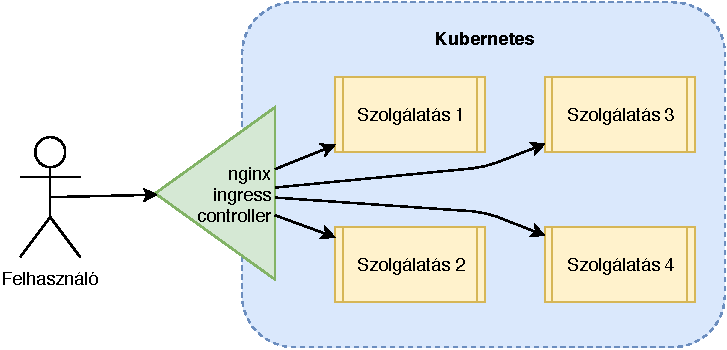
\includegraphics[width=110mm, keepaspectratio]{img/nginx_controller.pdf}
\caption{A Ingress Controller működése}
\end{figure}
\vskip 0.1in
A telepítés összesen két parancsot igényel mivel egyedi konfigurációt csak az Ingressek fognak tartalmazni. Az alábbi utasításokat adjuk ki:
\begin{lstlisting}
kubectl apply -f https://raw.githubusercontent.com/kubernetes/ingress-nginx/master/deploy/static/mandatory.yaml
kubectl apply -f https://raw.githubusercontent.com/kubernetes/ingress-nginx/master/deploy/static/provider/aws/service-nlb.yaml
\end{lstlisting}
Ezzel el is készült egy Elastic Network Load Balancer (NLB). Minden ide érkező kérést a megfelelő Podnak továbbít a vezérlő. De mi is az az "ide"? Az alábbi paranccsal nézzük meg:
\begin{lstlisting}
kubectl get services -n ingress-nginx

nginx-ingress-controller   LoadBalancer   10.100.253.39   ac...21.elb.eu-central-1.amazonaws.com 
80:32645/TCP,443:30928/TCP
\end{lstlisting}
A lényeg a \textbf{xxx.elb.yyy.amazonaws.com} cím. Erre célszerű úgynevezett CNAME-t felvenni a DNS\footnote{Domain Name System - domainok nevét fordítja IP címre} rekordok közé. A CNAME gyakorlatilag egy domaincímről egy másikra hivatkozó bejegyzés, melyet könnyű felismerni. Esetemben például így néz ki:
\begin{lstlisting}
host webshop.mbraptor.tech

webshop.mbraptor.tech is an alias for szakdolgozat.mbraptor.tech.
szakdolgozat.mbraptor.tech is an alias for ac...21.elb.eu-central-1.amazonaws.com.
ac...21.elb.eu-central-1.amazonaws.com has address 3.125.68.208
\end{lstlisting}
Azért van szükség erre, és nem közvetlenül az IP címre hivatkozni, mert az egy változó cím. Ezért ad az Amazon egy fix bejegyzést amit karban tart. Az \lstinline{mbraptor.tech} a saját domainem, melynek konfigurációját én kezelem.
Tehát elértük, hogy a szolgáltatásaink elérhetőek legyenek az internet felől. Azonban a klaszterünkben még semmi nem fut, csupán egy "404 Nem található" hibaüzenetet kapunk.
\section{Monitorozás kialakítása}
Monitorozás alatt most magának a klaszternek a monitorozását értem (bár a szolgáltatások erőforráshasználatára ez például tökéletesen alkalmas). Ezt végtelenül egyszerű lesz telepíteni a \textit{Helm} segítségével, ami lényegében egy Kubernetes csomagkezelő. Ezt viszont telepíteni kell a számítógépünkre:
\begin{lstlisting}
curl https://raw.githubusercontent.com/helm/helm/master/scripts/get-helm-3 > get_helm.sh
chmod 700 get_helm.sh
./get_helm.sh
\end{lstlisting}
A parancs futtatása után zárjuk be a terminálablakot és nyissuk meg újra. A Helm használatra kész.

Innen a fentebb ismertetett Prometheus monitorozó rendszer telepítése szó szerint két sor:
\begin{enumerate}
    \item Csináljunk egy namespacet a monitorozással kapcsolatos szolgáltatásoknak: \lstinline{kubectl create namespace monitoring}
    \item Telepítsük a Prometheust: \lstinline{helm install --name prometheus stable/prometheus --namespace monitoring}
\end{enumerate}

Most már a klaszterről tárolódnak a metrikák, azonban még megtekinteni nem lehet azt (legalábbis felhasználóbarát felületen nem). Ehhez a Grafana webalkalmazásra lesz szükség, melynek telepítése szintén egyszerű, de többletkonfigurációt igényel. Egyrészt be kell állítani adatforrásnak a Prometheust, illetve konfigurálni kell a Grafana perzisztenciát (hogy az esetleges módosítások ne tűnjenek el ha a Pod áthelyeződik). Ehhez két fájlt kell létrehozni az alábbi tartalommal:

grafana.yaml
\begin{lstlisting}
apiVersion: v1
kind: ConfigMap
metadata:
  name: prometheus-grafana-datasource
  namespace: monitoring
  labels:
    grafana_datasource: '1'
data:
  datasource.yaml: |-
    apiVersion: 1
    datasources:
    - name: Prometheus
      type: prometheus
      access: proxy
      orgId: 1
      url: http://prometheus-server.monitoring.svc.cluster.local
\end{lstlisting}
grafana-values.yaml
\begin{lstlisting}
sidecar:
  datasources:
    enabled: true
    label: grafana_datasource

persistence:
  enabled: true
  storageClass:
  annotations: {}
  accessMode: "ReadWriteOnce"
  size: "8Gi"
\end{lstlisting}
Illetve definiálnunk kell egy Ingress-t is, hogy melyik cím legyen a Grafanára irányítva. Én konfiguráltam a HTTPS kapcsolatot is, ez ugyan nem szükséges, de éles rendszerben ajánlott. Természetesen a tanúsítványt nem teszem közzé, azt fájlból is hozzá lehet adni, vagy base64 enkódolással a konfigurációba írni helyezni azt.

ingress.yaml
\begin{lstlisting}
apiVersion: networking.k8s.io/v1beta1
kind: Ingress
metadata:
  name: monitoring
  annotations:
    kubernetes.io/ingress.class: "nginx"
    nginx.ingress.kubernetes.io/force-ssl-redirect: "true"
spec:
  tls:
  - hosts:
    - szakdolgozat-monitoring.mbraptor.tech
    secretName: tls-mbraptor.tech
  rules:
  - host: szakdolgozat-monitoring.mbraptor.tech
    http:
      paths:
      - backend:
          serviceName: grafana
          servicePort: 80

---

apiVersion: v1
kind: Secret
data:
  tls.crt: ...
  tls.key: ...
metadata:
  name: tls-mbraptor.tech
type: kubernetes.io/tls
\end{lstlisting}
Ezeket a fájlokat már csak alkalmazni kell a \lstinline{kubectl apply -n monitoring -f FILENAME.yaml} paranccsal. Ha mindent jól csináltunk akkor a beállított oldalon (esetemben \url{szakdolgozat-monitoring.mbraptor.tech}) már elérhető a Grafana, a Helm telepítés végén található adminisztrátori adatokkal beléphetünk. A Grafana beállítása szakdolgozatomnak nem témája, de a \textit{Dashboard import} funkcióval és az \url{https://grafana.com/grafana/dashboards} oldalon található kész elrendezések jó kiindulási alapot jelenthetnek.
\section{Jenkins telepítése}
A Jenkins telepítését szintén Helm segítségével fogjuk végezni, azonban itt nagyobb mértékű konfigurációra lesz szükség. Egyrészt mivel a Jenkins közvetlenül fogja a Kubernetes API-t hívni ezért jogosultságokat kell adni neki, továbbá az alapértelmezett Jenkins konténerkép helyett is sajátot használok, illetve a fentebb beállított IAM szerepet is fel kell konfigurálni az AWS API kommunikációhoz.

Kezdetnek adjunk jogosultságot a Jenkinsnek. Ennek hozzunk létre egy fájlt péládul \lstinline{eks-jenkins-rbac.yaml} néven:
\begin{lstlisting}
kind: ClusterRole
apiVersion: rbac.authorization.k8s.io/v1
metadata:
  name: jenkins-role-cluster
rules:
- apiGroups:
  - ""
  - "apps"
  - "networking.k8s.io"
  - "autoscaling"
  resources:
  - pods
  - configmaps
  - deployments
  - secrets
  - services
  - ingresses
  - apps
  - horizontalpodautoscalers
  - statefulsets
  verbs:
  - create
  - delete
  - deletecollection
  - get
  - list
  - patch
  - update
  - watch

---

apiVersion: rbac.authorization.k8s.io/v1
kind: RoleBinding
metadata:
  name: jenkins-role-prod
  namespace: webshop-prod
roleRef:
  apiGroup: rbac.authorization.k8s.io
  kind: ClusterRole
  name: jenkins-role-cluster
subjects:
- kind: ServiceAccount
  name: ci-jenkins
  namespace: szakdolgozat-aws

---

apiVersion: rbac.authorization.k8s.io/v1
kind: RoleBinding
metadata:
  name: jenkins-role-beta
  namespace: webshop-beta
roleRef:
  apiGroup: rbac.authorization.k8s.io
  kind: ClusterRole
  name: jenkins-role-cluster
subjects:
- kind: ServiceAccount
  name: ci-jenkins
  namespace: szakdolgozat-aws
  ...
\end{lstlisting}
Mivel a Jenkins több névtérben is dolgozik, így egy klaszterszintű jogosultságot definiálunk (\textit{ClusterRole}), és ezt érvényesítjük adott névterekre (\textit{RoleBinding}), jelen esetben az alkalmazás két névterére.
Hozzuk létre a szóban forgó namespaceket és alkalmazzuk a konfigurációt:
\begin{lstlisting}
kubectl create namespace szakdolgozat-aws #ennek az elnevezésnek történelmi okai vannak, természetesen lehet jenkins is a neve
kubectl create namespace webshop-beta
kubectl create namespace webshop-prod

kubectl apply -n szakdolgozat-aws -f eks-jenkins-rbac.yaml
\end{lstlisting}
Ezzel a Kubernetes felé történő kommunikáció engedélyezve van, és a Jenkins által használt műveletek engedélyezve vannak (de természetesen ez alkalmazásfüggő). Szükséges még egy Ingress is: teljesen ugyanazt a műveletet kell elvégezni, amit a Grafana esetében (értelemszerűen a cím átírandó). Mivel konfigurált Jenkinst szeretnénk így a Helm telepítés előtt el kell készítenünk azt. Töltsük le az alábbi fájlt: \url{https://github.com/helm/charts/tree/master/stable/jenkins} és mentsük el \lstinline{jenkins-values.yaml} néven. Írjunk át benne pár dolgot:
Módosítsuk az alábbiakat, hogy az általam készített \textit{kubectl} és \textit{docker} klienssel ellátott konténerképet használja a telepítés.
\begin{lstlisting}
...
master:
  # Used for label app.kubernetes.io/component
  componentName: "jenkins-master"
  image: "msbence/jenkins-docker-kubectl"
  tag: "aws"
...
\end{lstlisting}
Adjuk hozzá környezeti változóként, hogy TCP kapcsolaton keresztül érjük el a Docker motort, továbbá adjuk meg azt az URL-t ahol a Jenkins elérhető lesz.
\begin{lstlisting}
...
initContainerEnv:
    - name: DOCKER_HOST
      value: "tcp://localhost:2375"
  containerEnv:
    - name: DOCKER_HOST
      value: "tcp://localhost:2375"
  # Set min/max heap here if needed with:
  # javaOpts: "-Xms512m -Xmx512m"
  # jenkinsOpts: ""
  jenkinsUrl: "https://ci.mbraptor.tech"
  # If you set this prefix and use ingress controller then you might want to set the ingress path below
...
\end{lstlisting}
Pár plugint telepítenünk kell az alapértelmezetteken túl. A \textit{BlueOcean} a Jenkins egy új, kísérleti felülete mely nagyban megkönnyíti annak használatát. A \textit{locale} plugin segítségével beállíthatunk nyelvet a szoftvernek ugyanis alapértelmezetten a böngésző által küldöttet használja, azonban a Jenkins magyar fordítása nem megfelelő minőségű. Az \textit{Amazon ECR} pedig a konténerképek feltöltésénél segít.
\begin{lstlisting}
...
  # List of plugins to be install during Jenkins master start
  installPlugins:
    - kubernetes:1.21.3
    - workflow-job:2.36
    - workflow-aggregator:2.6
    - credentials-binding:1.20
    - git:4.0.0
    - blueocean:1.19.0
    - locale:1.4
    - amazon-ecr:1.6
...
\end{lstlisting}
Fentebb hivatkoztunk egy Docker motorra melyet ez a konténer valósít meg. Ez egy \textit{Docker-in-Docker} konténerkép a hivatalos Docker csapat által támogatva.
\begin{lstlisting}
...
sidecars:
    configAutoReload:
    ...
    other:
     - name: docker-daemon
       image: docker:18.09-dind
       resources:
        requests:
          cpu: 50m
          memory: 512Mi
        limits:
          cpu: 2000m
          memory: 2048Mi
       securityContext:
           privileged: true
       volumeMounts:
                 - name: docker-graph-storage
                   mountPath: /var/lib/docker
...
\end{lstlisting}
Ahhoz hogy ne lássuk a gazdagép (Kubernetes worker node) Docker adatait egy üres tárolót kell csatolnunk, ezzel elfedve azokat.\cite{dind_ci}
\begin{lstlisting}
...
persistence:
  enabled: true
  existingClaim:
  storageClass:
  annotations: {}
  accessMode: "ReadWriteOnce"
  size: "8Gi"
  volumes:
      - name: docker-graph-storage
        emptyDir: {}
networkPolicy:
...
\end{lstlisting}
Ahhoz hogy a Pod hozzáférjen az AWS APIhoz a megfelelő szerepet kell kapnia. A fentebb létrehozott JenkinsRole szerepet állítsuk be az alábbi módon:
\begin{lstlisting}
...
rbac:
  create: true
  readSecrets: false

serviceAccount:
  create: true
  # The name of the service account is autogenerated by default
  name:
  annotations:
    eks.amazonaws.com/role-arn: "arn:aws:iam::123456789:role/JenkinsRole"

serviceAccountAgent:
...
\end{lstlisting}
A konfigurálást befejeztük, most már tényleg csak a Helm telepítést kell lefuttatni és szinte kulcsrakész Jenkinst kapunk fáradozásainkért cserébe. A parancs a Grafanához hasonló: \lstinline{helm install --name ci --namespace szakdolgozat-aws stable/jenkins -f jenkins-values.yaml}

Kis idő elteltével a Jenkins elérhető az Ingressnél megadott címen, az adminisztrátori jelszó megszerzéséről pedig a Helm tájékoztat. Belépés után a Jenkins kezelése (\textbf{Manage Jenkins}) menüben keressük meg a \textbf{Locale} plugin részét a \textbf{Rendszer kezelése} pont alatt és állítsuk a nyelvet \lstinline{en_US}-ra, valamit jelöljük be a \textbf{Ignore browser preference and force this language to all users} jelölőnégyzetet. Kattintsunk az \textbf{Apply} gombra és most már angol nyelvű felület fogad minket.

További hasznos teendő ha a \textbf{Manage Jenkins} menü alatt a \textbf{Global Security} menüben a \textbf{Security Realm}ot átállítjuk a Jenkins saját adatbázisára, ekkor lesz lehetőségünk több felhasználót hozzáadni, jelszót cserélni, stb...

Annak érdekében, hogy a Jenkins Docker támogatását könnyen használni tudjuk még be kell állítanunk az ECR hozzáférést is. Ezt bal oldalt a Credentials fül System almenüjében tehetjük meg a Global credentialshoz hozzáadva egy AWS Credential típusú hozzáférést:
\begin{itemize}
    \item \textbf{Scope}: Global
    \item \textbf{ID}: aws (vagy amit szeretnénk)
    \item \textbf{Description}: Ide tetszőleges leírást írhatunk
    \item \textbf{Access Key ID}: Felhasználóhoz tartozó hozzáférési azonosító
    \item \textbf{Secret Access Key}: A fenti azonosítóhoz tartozó tikos kulcs
\end{itemize}
Mentsük el a titkot és egyenlőre végeztünk a Jenkins beállításával, ugyanis az alkalmazást is konfigurálni kell.
\section{Alkalmazás konfigurálása Kuberneteshez}
Ahhoz hogy alkalmazás működjön Kubernetes alatt ahhoz létre kell hozni számára a megfelelő Kubernetes objektumokat. Első lépésben rendelkezésre kell álljon a konténerkép-tárolóban egy alkalmazáshoz tartozó kép. Szükséges továbbá konfigurálni egy \textit{Deployment}et mely később nyer értelmet, előljáróban annyit érdemes róla tudni, hogy több Podot fog össze ezzel biztosítva többek között a magas rendelkezésreállást. Szükséges továbbá egy Deploymenthez tartozó Service ami a hálózati (és Deploymentek közötti) kommunikációt teszi lehetővé, továbbá ha kívülről is el akarjuk érni a szolgáltatást akkor egy Ingress konfigurálása is szükséges. A további pontokban bővíteni fogjuk a konfigurációt, de az alapvető objektumok konfigurációja így néz ki (\textit{a következő példákat a backend alkalmazáson keresztül mutatom be}):
\begin{lstlisting}
apiVersion: networking.k8s.io/v1beta1
kind: Ingress
metadata:
  name: backend
  annotations:
    kubernetes.io/ingress.class: "nginx"
    nginx.ingress.kubernetes.io/force-ssl-redirect: "true"
spec:
  tls:
  - hosts:
    - webshop-api.mbraptor.tech
    secretName: tls-mbraptor.tech
  rules:
  - host: webshop-api.mbraptor.tech
    http:
      paths:
      - backend:
          serviceName: backend
          servicePort: 8081

---

apiVersion: v1
kind: Service
metadata:
  name: backend
  labels:
    run: backend
spec:
  ports:
  - port: 8081
    targetPort: 8081
    protocol: TCP
  selector:
    run: backend

---

apiVersion: apps/v1
kind: Deployment
metadata:
  name: backend
spec:
  selector:
    matchLabels:
      run: backend
  replicas: 2
  template:
    metadata:
      labels:
        run: backend
    spec:
      containers:
      - name: backend
        image: 794178227749.dkr.ecr.eu-central-1.amazonaws.com/webshop-backend:$IMAGE_TAG
        ports:
        - containerPort: 8081
        resources:
          requests:
            cpu: 100m
            memory: 256Mi
\end{lstlisting}
Az Ingress résznél definiálni kell az elérni kívánt szolgáltatás nevét, a kívülről elérhető címet, illetve a port számát amin a szolgáltatás elérhető klaszteren belülről. A szolgáltatásnál a lényeges beállítások a port, amin a szolgáltatás figyel, illetve a protokoll amit kommunikációra használ. A Deploymentnél kell megadni magát a konténerkép(ek)et amit futtatni szeretnénk, a portokat amit az adott konténer kommunikációra használ, illetve az erőforráskérelmet. A \lstinline{replicas} mező a futtatandó podok számát adja meg, célszerű legalább kettőt futtatni ha esetleg az egyikkel hiba történne akkor se legyen elérhetetlen a szolgáltatás.

\textit{Megjegyzés: a fenti .yaml konfigurációs fájl nem szabályos, azt "kézzel", kubectl segítségével nem lehet alkalmazni. A konténerkép specifikálásnál az \$IMAGE\_TAG egy változó, amit nem támogat a kubectl. Ezt a Jenkinsfileban fogjuk cserélni egy valós értékre.}

\subsection{Monitorozás}
A Kubernetes lehetőséget ad a szolgáltatások alapvető monitorozására kétféle módszerrel, mely két külön dologra alkalmas.
\begin{enumerate}
    \item \textbf{Readiness Probe} - Ez az ellenőrzés azt a célt szolgálja, hogy a Kubernetes tisztában legyen azzal, hogy egy Pod mikor lépett olyan állapotba amikor már képes kiszolgálni a kéréseket. Például a frissítések úgynevezett \textit{Rolling Update}tel történnek ami azt jelenti, hogy egy új pod indul, aztán egy régi törlődik, ez pedig addig zajlik így míg kizárólag új podok nem futnak. Azonban ha az alkalmazásnak hosszabb ideig tart megkezdeni a kiszolgálást akkor könnyen előfordulhat, hogy már az összes Pod le lett cserélve de azok közül egyik sem szolgál ki.
    \item \textbf{Liveness Probe} - Ez az ellenőrzés hasonlít az előbbire azonban ez a már elindult szolgáltatást ellenőrzi hogy képes-e még kiszolgálni a kéréseket. Ha hibát észlel a Podon akkor leállítja azt, majd indít egy újabb példányt.
\end{enumerate}
Bővítsük ki a Deployment konfigurációját:
\begin{lstlisting}
...
        - containerPort: 8081
        readinessProbe:
          httpGet:
             path: /api
             port: 8081
          initialDelaySeconds: 5
          periodSeconds: 5
          successThreshold: 1
        livenessProbe:
          httpGet:
             path: /api
             port: 8081
          initialDelaySeconds: 10
          periodSeconds: 30
          successThreshold: 1
        resources:
...
\end{lstlisting}
Ez engedélyezi a monitorozást egy egyszerű módszer segítéségvel. A backend a \lstinline{/api} útvonalon nyújt szolgáltatást HTTP segítségével. Gyakorlatilag ezt nézi időközönként a klaszter, hogy érkezik-e vissza válasz, és ha igen akkor az megfelelő-e (tehát HTTP 200 OK).
\subsection{Skálázás}
A Kubernetes képes monitorozni a benne futó komponensek erőforráshasználatát és a konfigurált értékek alapján skálázni azokat amennyiben szükséges. Az Amazon EKS alapértelmezésben nem telepíti a \lstinline{metrics-server} összetevőt, így ha mégis szükségünk van rá (\textit{nekünk a skálázás megvalósításához szükséges, ez a komponenes szolgáltat erőforrás-adatokat a Kubernetes API számára}) akkor követnünk kell a dokumentációt\cite{metrics_eks} miszerint pár paranccsal ez elvégezhető:
\begin{lstlisting}
DOWNLOAD_URL=$(curl -Ls "https://api.github.com/repos/kubernetes-sigs/metrics-server/releases/latest" | jq -r .tarball_url)
DOWNLOAD_VERSION=$(grep -o '[^/v]*$' <<< $DOWNLOAD_URL)
curl -Ls $DOWNLOAD_URL -o metrics-server-$DOWNLOAD_VERSION.tar.gz
mkdir metrics-server-$DOWNLOAD_VERSION
tar -xzf metrics-server-$DOWNLOAD_VERSION.tar.gz --directory metrics-server-$DOWNLOAD_VERSION --strip-components 1
kubectl apply -f metrics-server-$DOWNLOAD_VERSION/deploy/1.8+/
\end{lstlisting}
Ezzel a komponens feltelepült, ellenőrizni a \lstinline{kubectl get deployment metrics-server -n kube-system} utasítással tudjuk.

Természetesen az alkalmazásunkat is konfigurálni kell, mégpedig egy \textit{Horizontal Pod Autoscaler} objektum hozzáadásval a konfigurációs .yaml fájlhoz:
\begin{lstlisting}
...
            memory: 256Mi

---

apiVersion: autoscaling/v1
kind: HorizontalPodAutoscaler
metadata:
  name: backend
spec:
  scaleTargetRef:
    apiVersion: apps/v1beta1
    kind: Deployment
    name: backend
  minReplicas: 2
  maxReplicas: 4
  targetCPUUtilizationPercentage: 50
\end{lstlisting}
Itt adjuk meg, a minimum és maximum értéket ami között skálázni lehet a példányok számát, továbbá azt is hogy milyen átlagos erőforráskihasználtságot szeretnénk tartani.
\subsection{Adatbázis replikációja}
A Postgres támogatja a replikációt, mely a skálázhatóság egyik kulcseleme. Ennek a menete pontosabban úgy működik, hogy van egy kitüntetett adatbázispéldány ami felé az írási kérelmek érkeznek, és ez a példány propagálja a többi alárendelt adatbázis felé az adatot, azokból kizárólag olvasni lehet. Ezt \textit{master-slave} replikációnak nevezik. Ebből fakadóan kizárólag az adatbázis olvasási teljesítménye növelhető több példány indításával. Az írási kapacitás növeléséhez a mesterpéldány számára kell több erőforrást allokálni.

Az adatbázis Kubernetesbe ültetéséhez egy már meglévő - nem általam készített - GitHub repositoryt\cite{postgres_k8s} vettem igénybe, és ezt ültettem át egy Jenkins segítségével építhető folyamatba.
\clearpage
A folyamat során az alábbi lépések zajlanak le:
\begin{figure}[ht]
\centering
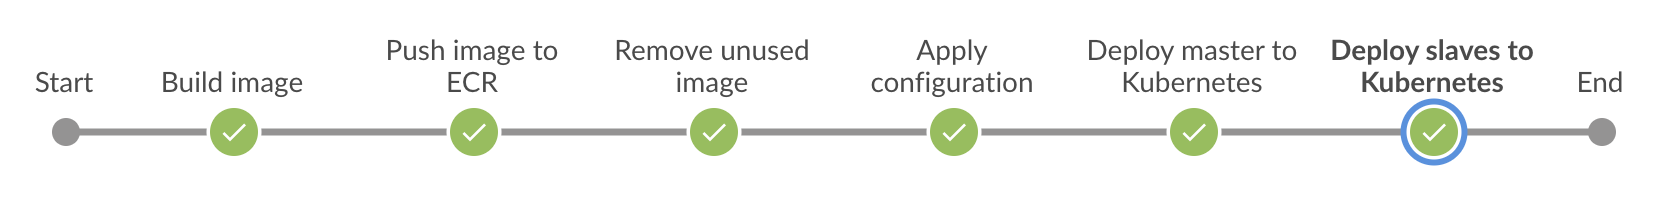
\includegraphics[width=150mm, keepaspectratio]{img/dbjenkins.png}
\caption{Az adatbázistelepítés Jenkinsben végrehajtott lépései}
\end{figure}
\vskip 0.1in
\begin{enumerate}
    \item \textbf{Konténerkép összeállítása} - Erre a lépésre azért van szükség mert egy \lstinline{init.sql} fájlt rá kell másolni a konténerre, így viszont már új kép keletkezik (\textit{megjegyzés: a kezdeti inicializálást Kubernetes ConfigMap segítségével is meg lehetne oldani. Számomra a Docker képfájl a lokális tesztelés során volt kényelmes}). Ezzel történik az adatbázis inicializálása az első telepítéskor (frissítés során értelemszerűen nem).
    \item \textbf{Konténerkép feltöltése ECRbe} - Ahhoz hogy a Kubernetes hozzáférjen az előbb épített képhez ahhoz ECRbe kell feltölteni.
    \item \textbf{Nem használt kép eltávolítása} - A Docker-in-Docker konténer megőrzi a képet alapértelmezetten. Ezt ki kell törölni hogy ne teljen meg a lemezterület. (Az ECR tárolja a képeket.)
    \item \textbf{Konfiguráció alkalmazása} - Ez alkalmazza a GitHub repositoryban található \textit{Secret} és \textit{ConfigMap} objektumokon végzett változtatásokat.
    \item \textbf{Mesterpéldány telepítése} - A mesterpéldányon végzett módosításokat lépteti érvénybe. Nem jár adatbáziskieséssel ugyanis az alárendelt példányok átveszik a mester szerepét a kiesés idejére.
    \item \textbf{Alárendelt példányok telepítése} - Miután a főpéldány újra készen áll a kiszolgálásra, az alárendelt példányok frissítése is megtörténik.
\end{enumerate}
Az adatbázison összesen a jelszavakat kell konfigurálni, a többi teljesen működőképes állapotba kerül a Jenkins segítségével. Ezt a \lstinline{secrets.yaml} fájlban lehet megtenni. Szükséges egy replikációs jelszó és egy hozzáférési jelszó is. Előbbi csak az adatbázispéldányok közti kommunikációra használatos, nem kell megjegyezni. Utóbbi az alkalmazások/emberek számára is látható, az adminisztrátori hozzáférést biztosítja a telepítés után.
\section{CI és CD megvalósítása}
A Jenkins készen áll arra hogy alkalmazásokat telepítsen Kubernetesbe, az alkalmazások pedig fel vannak erre készítve. Már csak azt kell megoldani hogy a Jenkins tudja, hogy \textit{honnan}, \textit{mikor} és \textit{hogyan} telepítse azokat.
\subsection{Jenkinsfájlok}
A Jenkinsben úgynevezett \textit{Multibranch pipeline} fog létrejönni amikor majd összekötjük a GitHubbal. Ezt azt jelenti, hogy alapértelmezetten amelyik git ágon egy \textit{Jenkinsfile} nevű fájl található, azt a Jenkins számára értelmezettnek tekinti és megkísérli végrehajtani az ott leírt utasításokat.

Egy Jenkinsfile szakaszokból, a szakaszok pedig lépésekből épülnek fel. Ezek a lépések párhuzamosan is végrehajthatóak (bár ez a feladatom során nem volt hasznosítható). Minden szakasznak definiálható továbbá hogy mikor hajtódjon végre. A lépések során használhatunk Docker parancsokat, futtathatunk Shell szkriptet, vagy egyéb szolgáltatásokat is igénybe vehetünk (mivel a Jenkins erősen bővíthető). Ismételten a backend példáján keresztül fogom szemlélteni a működést:
\begin{lstlisting}
def branch_name = "${BRANCH_NAME}" //a branch nevét környezeti változóból groovy változóba helyezzük későbbi használatra
pipeline {
  environment {
    //meghatározzuk a használni kívánt registryt és repositoryt
    registry = "XXXXXXXXXXX.dkr.ecr.eu-central-1.amazonaws.com/webshop-backend"
    registryCredential = 'ecr:eu-central-1:aws' //ez az Amazon hozzáférés amit korábban a Jenkinsben elmentettünk. Formátum: ecr:régió:credential_ID
    dockerImage = '' //ez majd a keletkezett konténerképet fogja tárolni
    IMAGE_TAG = "$BUILD_NUMBER-$BRANCH_NAME" //a konténer tagje lesz a build sorszáma és a branch neve
    NAMESPACE = "webshop-$BRANCH_NAME" //a névtér amibe a kubernetesen belül telepíteni fogunk
    DOMAIN = "mbraptor.tech" //ez a változó később a yaml fájlba fog kerülni
  }
  agent any
  stages {
    stage('Build image') {
      steps{
        script {
          dockerImage = docker.build registry + ":$IMAGE_TAG" //beépített paranccsal konténerképet készítünk
        }
      }
    }
    stage('Push image to ECR') {
      when {
        expression { return branch_name ==~ /(prod|beta)/ } //ha a kitüntetett branch valamelyikén vagyunk csak akkor hajtjuk végre ez a szakaszt
      }
      steps{
        script {
          docker.withRegistry("https://" + registry, registryCredential) {
            dockerImage.push() //adott belépési adatokkal feltöltjük ECRbe a képet
          }
        }
      }
    }
    stage('Remove unused image') {
      when {
        expression { return branch_name ==~ /(prod|beta)/ }
      }
      steps{
        sh(script: "docker rmi $registry:$IMAGE_TAG", returnStdout: true) // töröljük a képet a lokális dockerből
      }
    }
    stage('Deploy to Kubernetes') {
      when {
        expression { return branch_name ==~ /(prod|beta)/ }
      }
      steps{
        sh(script: "envsubst < backend-${BRANCH_NAME}.yaml | kubectl -n $NAMESPACE apply -f - && sleep 10", returnStdout: true) //a változókat a linuxos envsubst program segítségével átírjuk az értékükre (pl.: \$IMAGE\_TAG), majd alkalmazzuk a Kubernetesben a változtatásokat
      }
    }
  }
}
\end{lstlisting}
Ha minden lépés sikerrel lezajlott akkor zöld színű lesz a Jenkins, ellenkező esetben piros, és hibaüzenetet kapunk.
\subsection{GitHub konfigurálása}
Ahhoz hogy a Jenkins példányunk a GitHubon tárolt forráskódhoz hozzáférjen ahhoz be kell konfigurálni egy-két dolgot. Az első lépés a hozzáférés engedélyezése.
Szükségünk lesz egy úgynevezett \textit{GitHub Personal Access Token}re mely gyakorlatilag egy egyszerű szövegfüzér. Ezt a GitHub oldalán a \textbf{Profile} gombra kattintva a \textbf{Settings} alatt a \textbf{Developer settings}nél találjuk. Itt kattintsunk a \textbf{Generate new token} gombra. Az alábbi jogosultságokat adjuk meg:
\begin{itemize}
    \item admin:repo\_hook
    \item read:user
    \item repo
    \item user:email
\end{itemize}
Ezzel kapunk egy hosszabb szöveget mely a token a Jenkins számára. Ezt két helyen kell felhasználni a Jenkinsen belül:
\begin{itemize}
    \item A \textbf{Manage Jenkins, Configure System} útvonalon keressük meg a \textbf{GitHub} részt. Adjunk hozzá egy \textbf{GitHub szerver}t tetszőleges névvel. Az \textbf{API URL} \url{https://api.github.com} a \textbf{Credentials}nál pedig adjunk hozzá egy új \textbf{Secret Text} típusú titkot és másoljuk be a tokent. Válasszuk ki a legördülő menüben az előbb létrehozott titok azonosítóját, illetve jelöljük be a \textbf{Manage Hooks} jelölőnégyzetet.
    \item Nyissuk meg a \textbf{Blue Ocean} nézetet mely a Jenkins új felülete, és válasszuk a \textbf{New Pipeline} lehetőséget. Itt menjünk végig a lépéseken, másoljuk be a tokent és válasszunk egy tetszőleges repositoryt.
\end{itemize}
Ezzel a kapcsolat létrejött a GitHub és a Jenkins között és a Manage Hooks bejelölése miatt a WebHook is megjelenik a GitHub repository megfelelő részén.

A webhookok segítségével a Jenkins valós időben értesül a feliratkozott eseményekről. Erről a GitHub HTTP \textit{POST} kérés formájában értesíti a megadott végpontot.
\begin{figure}[ht]
\centering
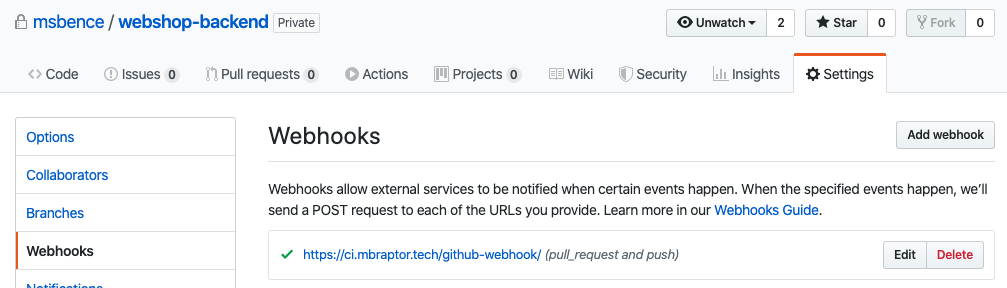
\includegraphics[width=150mm, keepaspectratio]{img/webhook.png}
\caption{A GitHub oldalon megjelenik az új webhook}
\end{figure}
\vskip 0.1in
A másik két alkalmazáskomponens felvétele a Blue Ocean felületen hasonlóan egyszerű.

Még két fontos dolgot kell beállítani, bár ez opcionális, és tervezés kérdése. Én a gyakorlatban alkalmazhatónak gondolom a lentieket, és szeretném megmutatni a lehetőségeket. Célszerű konfigurálni a Jenkins feladatnál, hogy kizárólag a kitüntetett ágakat és a Pull Requesteket vegye figyelembe. Természetesen ahogyan az Jenkinsfileban is látszik, a telepítési/frissítési feladatok ettől a beállítástól függetlenül, kizárólag csak a két főágon hajtódnak végre. Válasszünk ki egy Jenkins feladatot a \textbf{hagyományos} felületen, ekkor bal oldalt megjelenik a \textbf{Configure} lehetőség. Itt válasszük a \textbf{Branch Sources} fület, és adjunk hozzá egy RegEx\footnote{Regular Expressions - reguláris kifejezések, gyakorlatilag egy szűrőkifejezés mely szövegre illetszthető} szűrőt a következő értékkel: \lstinline{(prod|beta|PR.+)} (tehát a \textit{prod} vagy \textit{beta} vagy a \textit{PR-} kezdetű branchek (a pull requestek a Jenkinsben PR-ként jelennek meg)).
\begin{figure}[ht]
\centering
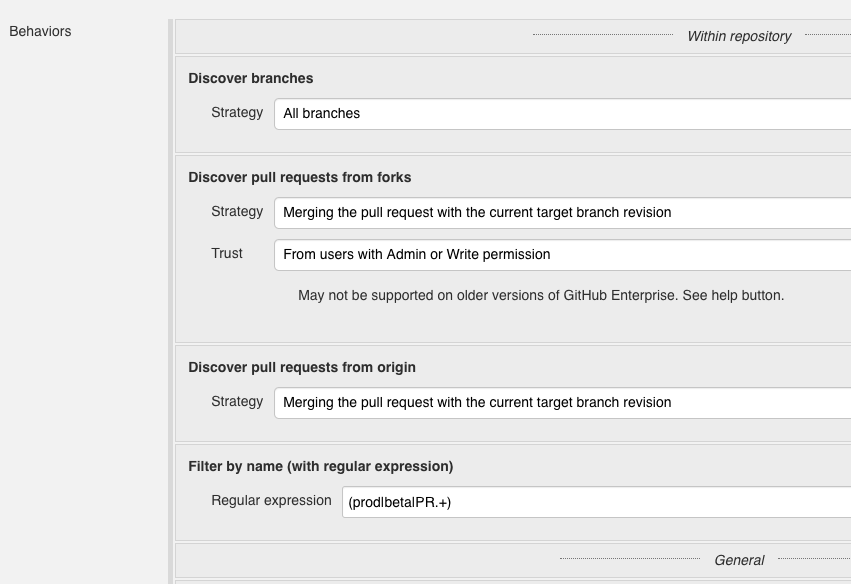
\includegraphics[width=150mm, keepaspectratio]{img/jenkinsbranch.png}
\caption{Ágak szűrése Jenkins és RegEx segítségével}
\end{figure}
\newpage
A másik hasznos lehetőség a korábban említett \textit{Branch Protection} alkalmazása. Ezt GitHubon kell konfigurálni egy adott repositoryn belül. A megfelelő beállításokkal "védetté" tehetjük az adott ágat, például csak akkor olvaszhatunk bele módosításokat, ha a Jenkins azt leellenőrizte. Konfigurálható még továbbá, hogy egy fejlesztőnek kötelező átnéznie azt. Ahhoz, hogy a Jenkins ellenőrzést kötelezővé tudjuk tenni, ahhoz a GitHubnak regisztrálnia kell annak létezését, amihez viszont egy Pull Requestnek léteznie kell. Csináljunk egyet, később törölhetjük, nem kell elfogadni sem. Most már látni fogja a GitHub a Jenkins ellenőrzés létezését, állítsuk is be. A repository \textbf{Settings} fülén válasszuk bal oldalt a \textbf{Branches} részt, és a \textbf{Branch Protection Rules}nál adjunk hozzá egy új szabályt az \textbf{Add rule} gombra kattintva. A \textbf{Branch name pattern}nél adjuk meg a védeni kívánt branch nevét (sajnos jelenleg áganként külön szabályt kell felvinni), és jelöljük be a \textbf{Require status checks to pass before merging} négyzetet, azon belül pedig a \textbf{Require branches to be up to date before merging} négyzetet. A Jenkins ellenőrzést a \textbf{continuous-integration/jenkins/pr-merge} bejelölésével kapcsolhatjuk be. Érdemes még engedélyezni a force pusht (\textbf{Allow force pushes}), ugyanis a Git használata során ez bizonyos esetekben (rebase) teljesen indokolt lehet.
\begin{figure}[ht]
\centering
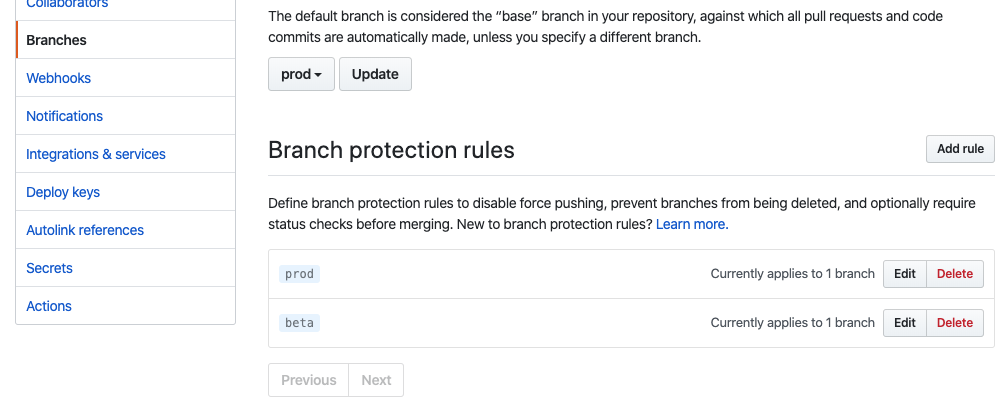
\includegraphics[width=150mm, keepaspectratio]{img/gitbranch.png}
\caption{Az fontos ágak védve vannak}
\end{figure}

Ezekkel a beállításokkal gyakorlatilag a feladat \textit{Continuous Integration} része is elkészült, most már biztosak lehetünk benne hogy az általunk választott ágakon kizárólag Jenkins által ellenőrzött kód található, az azzal való munka során egészen biztosan egy működő állapotból indulunk ki.
\newpage
\subsection{Alkalmazás telepítése és frissítése}
Miután a fentieket az összes alkalmazáskomponenesre elvégeztük gyakorlatilag végeztük is. Ha mindent jól csináltunk, akkor amikor a Jenkinsbe regisztráltuk a GitHub repositorykat akkor az végrehajtotta az összes lépést és ez a telepítést is magában foglalja. Innentől kezdve ha egy Pull Request (\textit{ami szintén ellenőrizve lesz, csupán a frissítéssel kapcsolatos lépések maradnak ki}) elfogadásra kerül, tehát a főágba lesz olvasztva akkor a Jenkins végrehajtja azon az ágon is a teljes folyamatot, azonban itt már minden lépést, tehát az alkalmazáskomponens frissítve lesz, mégpedig leállás nélkül, tekintettel arra, hogy minden egységnél definiáltunk \textit{Readiness Probe}ot, a Kubernetes pedig alapértelmezésben egyesével cseréli a futó példányokat. Ezzel elkészült egy teljes CI/CD alkalmazás.
\begin{figure}[ht]
\centering
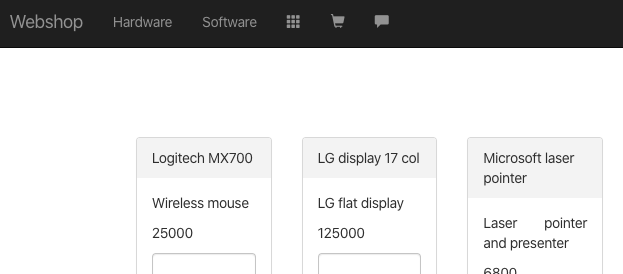
\includegraphics[width=120mm, keepaspectratio]{img/appprod.png}
\vskip 0.2in
%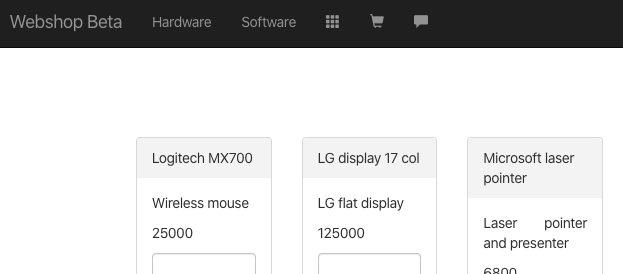
\includegraphics[width=120mm, keepaspectratio]{img/appbeta.png}
%\vskip 0.2in
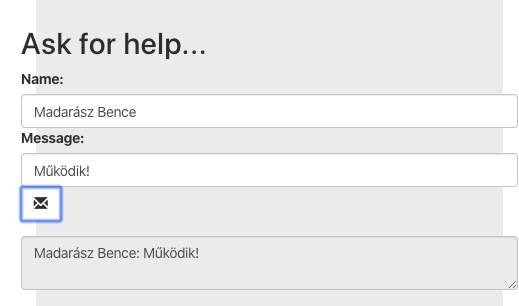
\includegraphics[width=120mm, keepaspectratio]{img/appchat.png}
\caption{A működő webáruház és chatfelülete}
\end{figure}
\chapter{Összegzés}
\section{Az elért eredmény}
Az alkalmazás beüzemelése sikerült, és büszke vagyok arra a megoldásra amit építettem. Három privát GitHub repositoryban található a három alkalmazáskomponens, mindegyiken külön dedikált \textit{prod} (az éles, felhasználók számára látható verzió), és \textit{beta} (fejlesztők számára, az élessel megegyező környezetben futó tesztverzió) ág. Mindkét ág \textit{branch protection}nel van ellátva, arra leadott pull request csak akkor fogadható el ha annak Jenkins buildje sikeresen lefutott.

CI/CD szempontjából sikerült elérni a várakozásokat. A GitHubbal koordináltan zajlik a kiemelt ágak és pull requestek ellenőrzése (más ágaké nem, a buildszerver indokolatlan leterheltségének megelőzése érdekében). Amennyiben a Jenkins sikeresen lebuildeli az alkalmazást, akkor a konténerképet privát ECR repositoryba küldi és alkalmazza a Kubernetesben a változtatásokat, lépcsőzetes frissítés segítségével. Ha valami a tesztek ellenére balul sülne el, akkor a deployment manuális szerkesztésével, a konténerkép verziószámának (ami a \textit{tag}je) átírásával gyorsan vissza lehet állni korábbi verzióra.
\begin{figure}[ht]
\centering
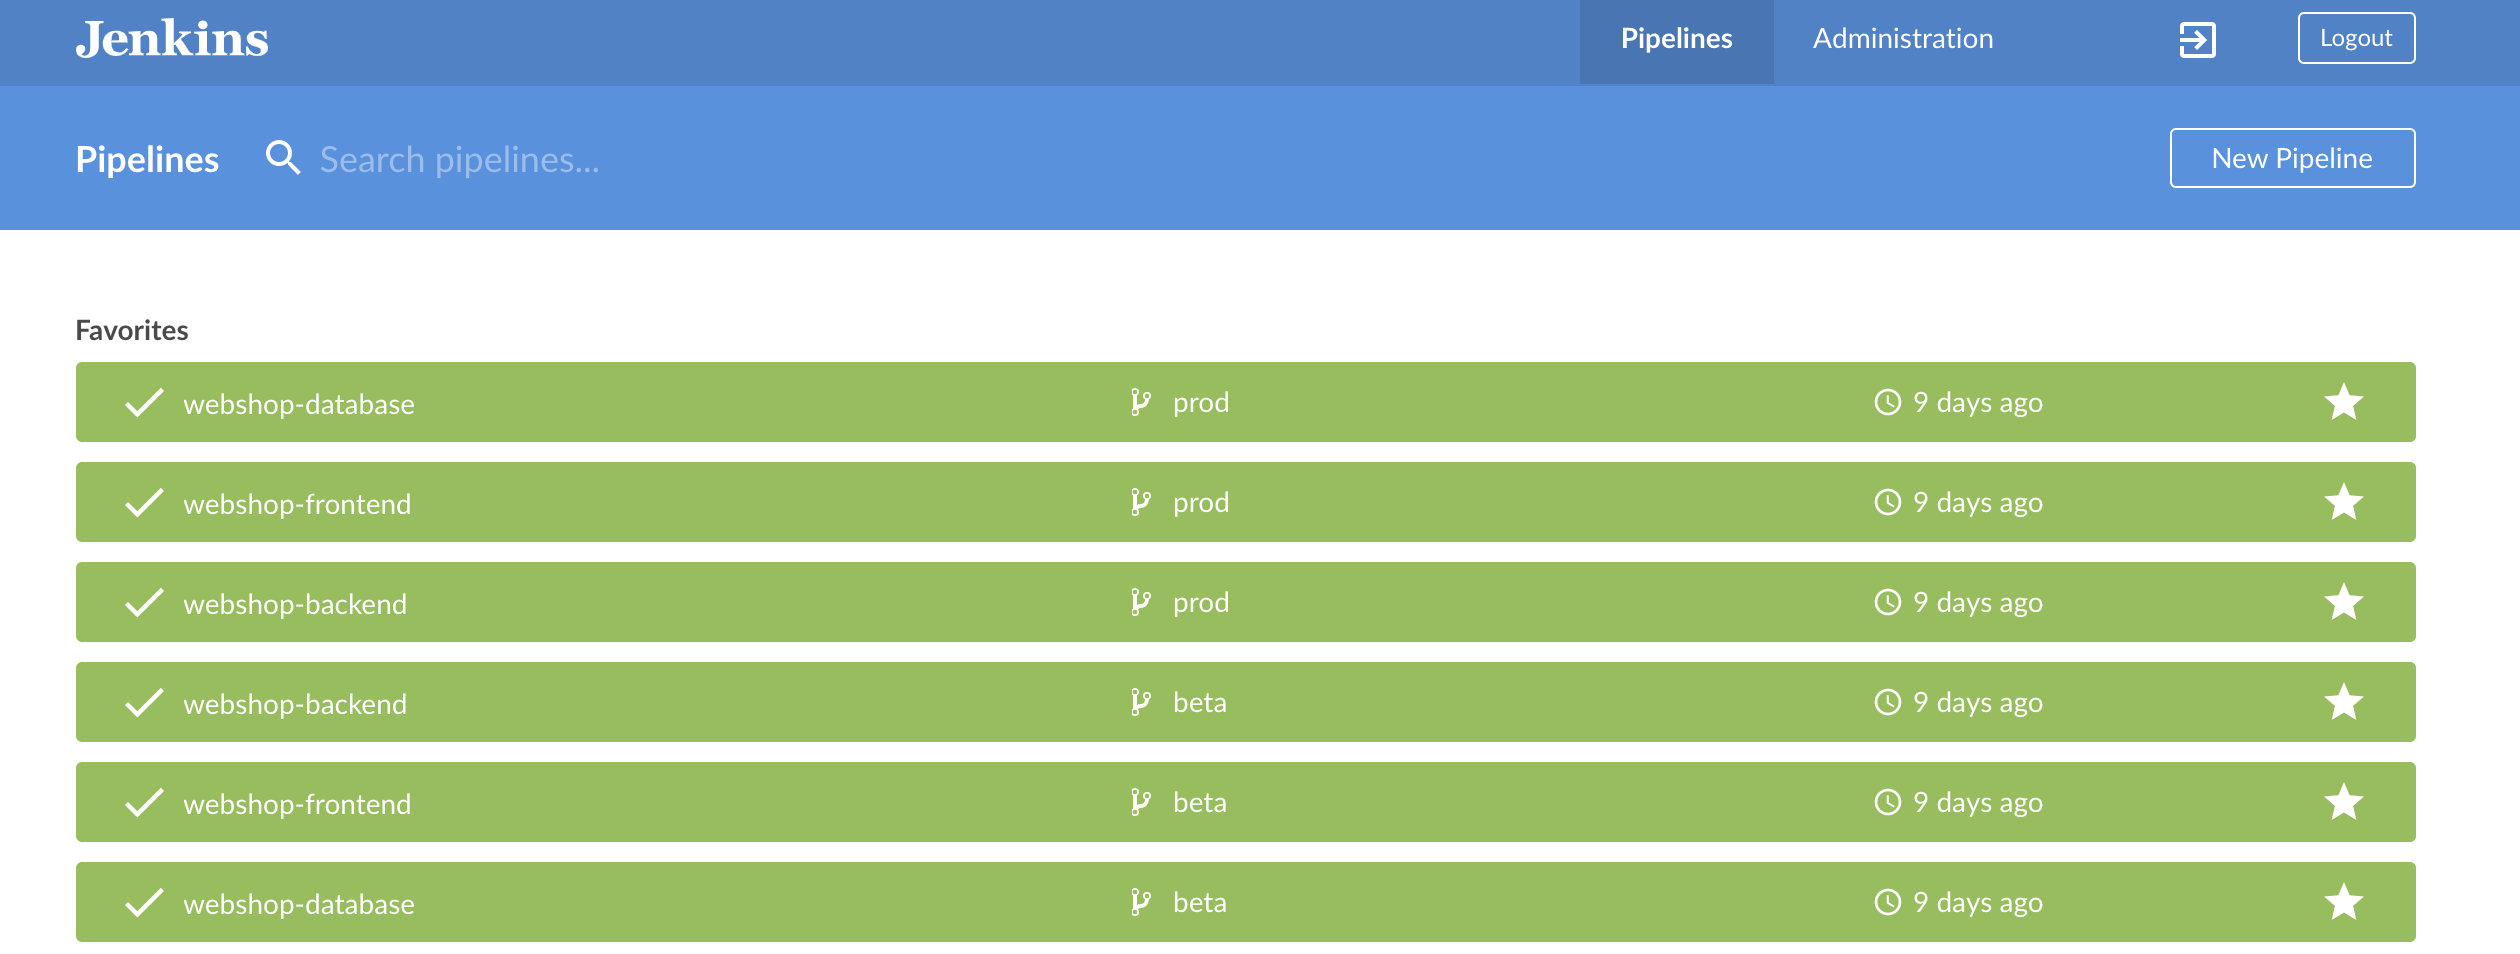
\includegraphics[width=150mm, keepaspectratio]{img/jenkinsgreen.png}
\caption{Minden ág sikeresen lefordul és települ}
\end{figure}
\vskip 0.1in
Az alkalmazás automatikusan skálázódik, mégpedig minden komponense. Egységesen 50\% CPU használatra van beállítva mindhárom rész. Az adatbázis az állapotfüggőségből adódóan nem skálázható teljesen: a Postgres úgynevezett \textit{master-slave replikáció}t használ, ami azt jelenti, hogy bár egyszerre több példányt is lehet olvasni, írni csak és kizárólag a mesterpéldányt lehet. A gyakorlatban tehát az adatbázisnak csak az olvasási teljesítménye skálázható, az írási kizárólag vertikálisan (azaz több erőforrás hozzáadásával) növelhető.
\clearpage
\begin{figure}[!ht]
\centering
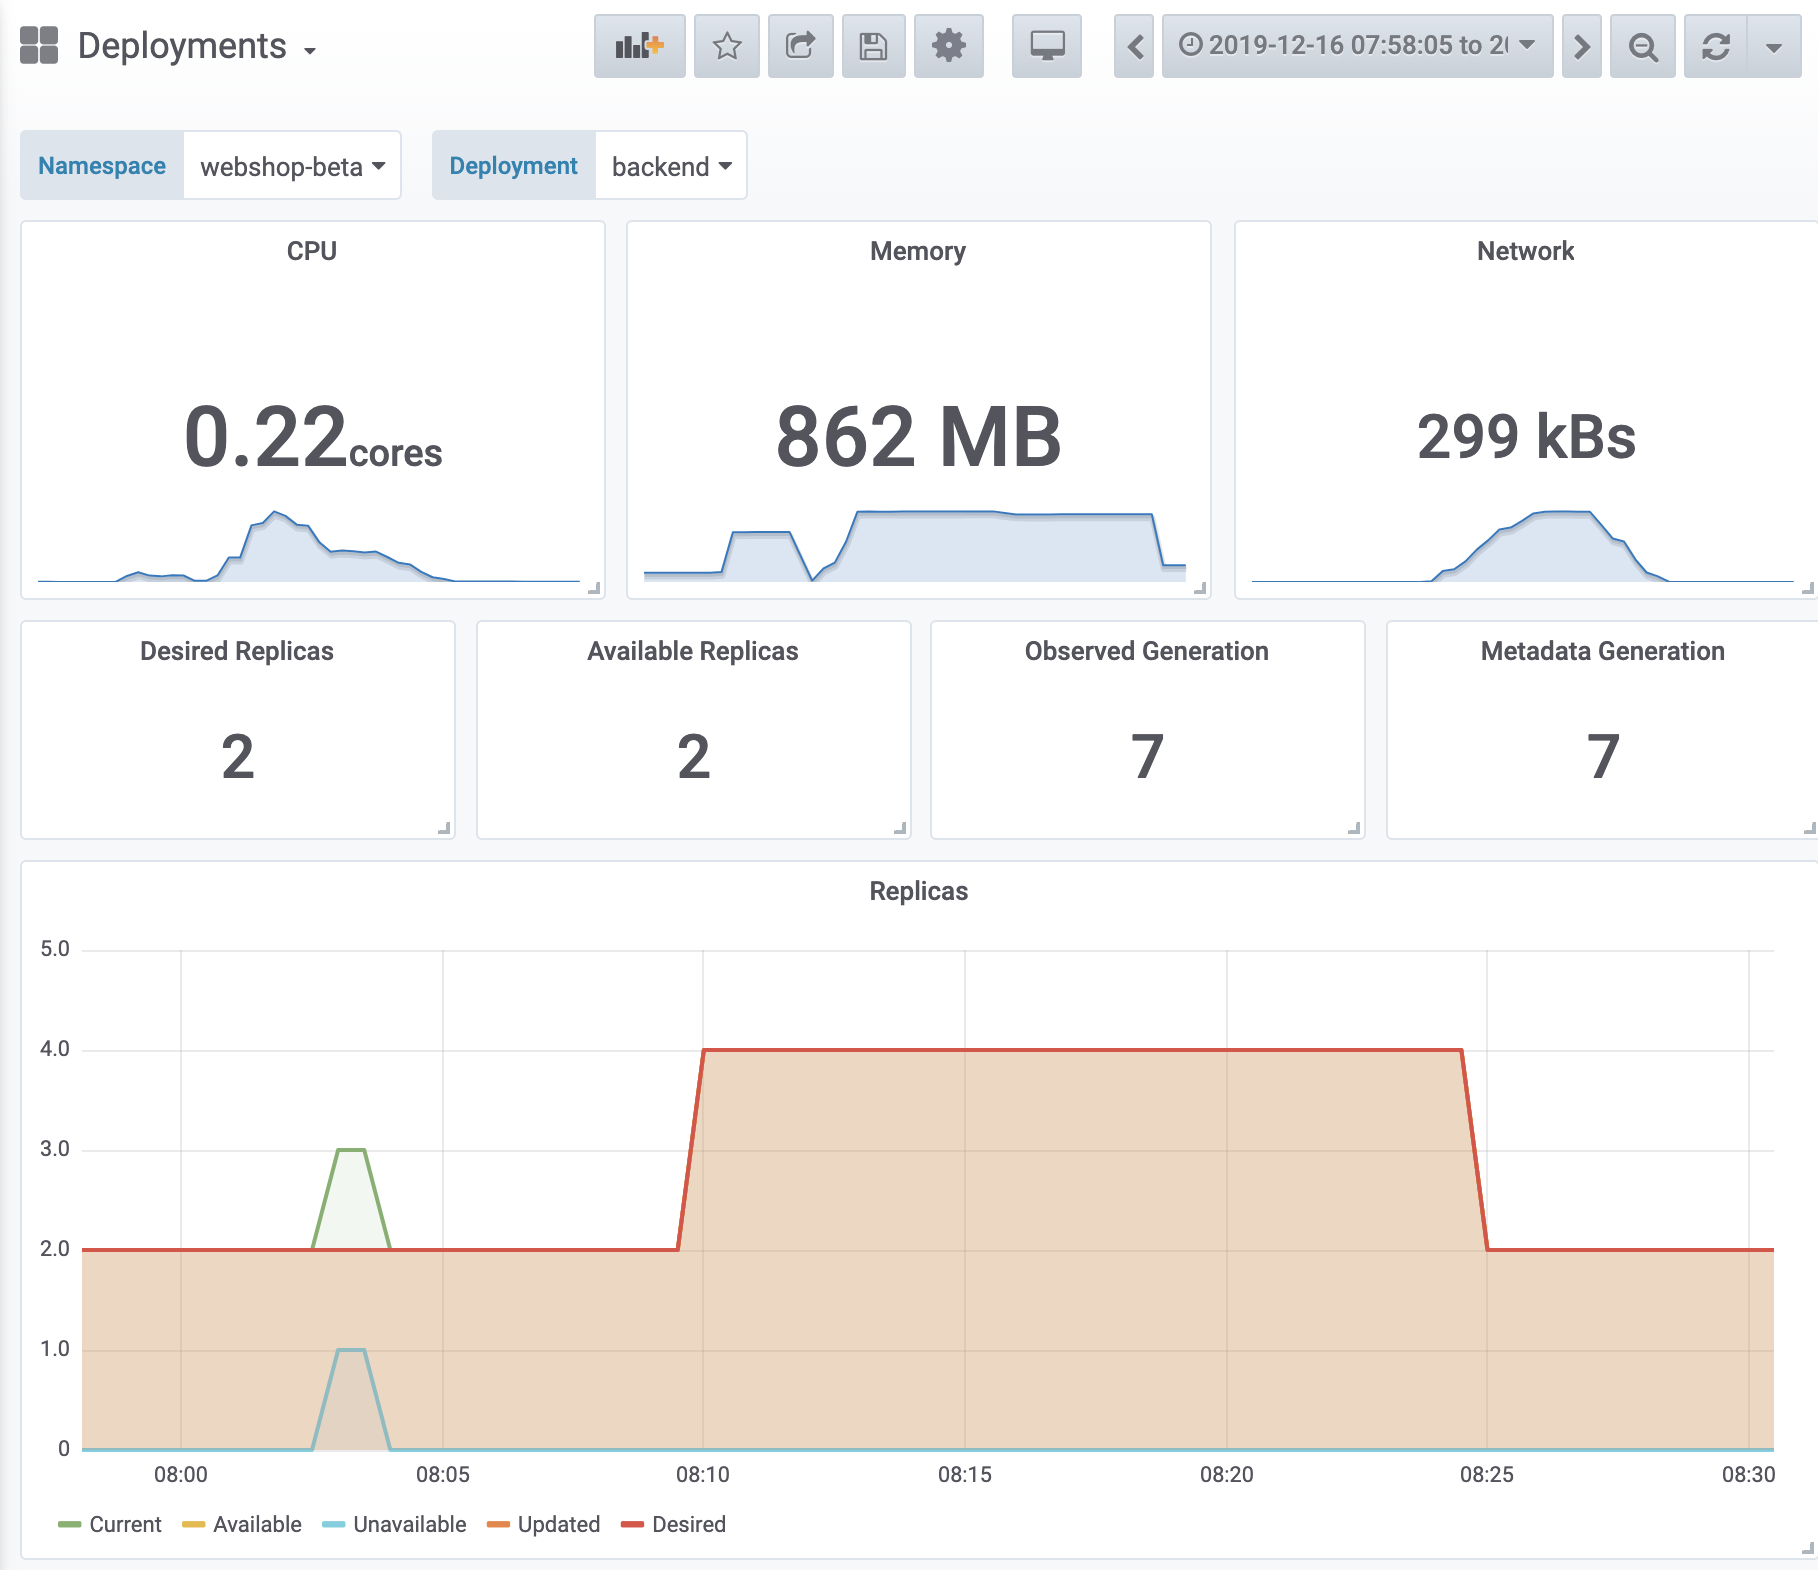
\includegraphics[width=150mm, keepaspectratio]{img/replica_up.png}
\vskip 0.5in
\vfill
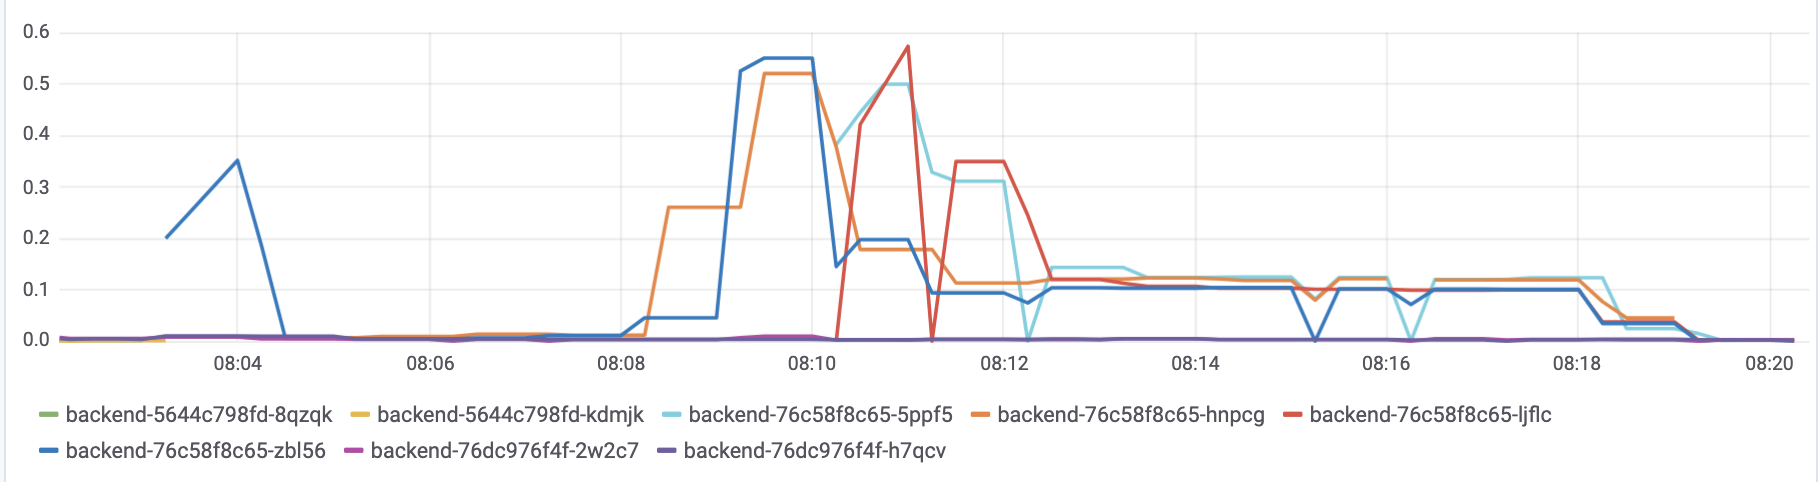
\includegraphics[width=150mm, keepaspectratio]{img/hpa_cpu.png}
\caption{Terhelés hatására új példányok indulnak, a processzorhasználat normalizálódik}
\end{figure}
\clearpage
Monitorozás szempontjából minden részkomponens a Kubernetes adta readiness és liveness ellenőrzésekkel el van látva (HTTP státuszkód 200 (OK) kell legyen a visszatérési státuszkód), ha meghibásodik valamelyik akkor az automatikusan törlésre kerül és új példány indul belőle. A magas rendelkezésreállás is garantált mivel minden komponens minimum két példányban fut. Ez az adatbázisra is igaz, ugyanis a mester halála esetén az alárendelt példány ideiglenesen átveszi a mester feladatát, írhatóvá válik, majd a mester újraéledése során visszaszinkronizálja az adatokat és minden visszaáll eredeti állapotába.
\section{Nehézségek}
Az első komoly kihívást előre sejtettem: állapotfüggő alkalmazást szerettem volna több példány indításával skálázni, az adatbázist. Ez egy meglehetősen bonyolult feladatnak bizonyult, ráadásul az eredetileg az alkalmazás által használt \textit{HyperSQL}-t nem ismertem. Kutatásom során rájöttem, hogy csak replikációt támogató adatbázissal megoldható a probléma, és azzal sem feltétlenül egyszerűen. Egy útmutató példa volt a népszerű MySQL Kubernetesbe helyezéséről szóló dokumentáció\cite{db_k8s}, és kis olvasás után rájöttem, hogy a számomra jobban ismert Postgres is skálázhatóvá tehető, ha csak olvasási teljesítményben is.

Egy másik probléma a Jenkins pipeline kialakításakor került elő: \textit{Multistage Dockerfile}ok segítségével fordítottam a projekteket, ami gyakorlati szempontból annyit jelent, hogy egy Docker motor elérhető kell legyen a Jenkins számára. Mivel én már magát a Jenkinst is Kubernetesben futtattam (ami pedig Dockerre épít), így egy érdekes megoldást választottam (és fenntartom, hogy nem ez a legoptimálisabb megoldás): Docker in Docker konténert is definiáltam a Jenkinshez tartozó Podba (\textit{emlékeztető: A Pod a Kubernetes legkisebb egysége, konténerek összessége}) majd a Jenkinsen átadtam a megfelelő \lstinline{DOCKER_HOST} környezeti változót, illetve egy egyedi Jenkins konténerképet csináltam, melybe többek között egy Docker klienst is elhelyeztem.

Hasonló problémába ütköztem a Kubernetesbe való alkalmazástelepítéskor is. Nem tudtam könnyedén kommunikálni a Kubernetes API-val ugyanis hiányzott a \textit{kubectl} nevű eszköz mely ezt a feladatot látja el. Szintén az egyedi konténerképben helyeztem el, ami elérhető DockerHubon\footnote{\url{https://hub.docker.com/repository/docker/msbence/jenkins-docker-kubectl} \newline msbence/jenkins-docker-kubectl:aws}. Az ehhez tartozó Dockerfile itt található:
\begin{lstlisting}
FROM jenkins/jenkins:lts
USER root
RUN apt-get update && \
apt-get -y install apt-transport-https \
     ca-certificates curl gnupg2 python3-pip \
     gettext \
     software-properties-common && \
curl -fsSL https://download.docker.com/linux/$(. /etc/os-release; echo "$ID")/gpg > /tmp/dkey; apt-key add /tmp/dkey && \
add-apt-repository \
   "deb [arch=amd64] https://download.docker.com/linux/$(. /etc/os-release; echo "$ID") \
   $(lsb_release -cs) \
   stable" && \
apt-get update && \
apt-get -y install docker-ce
RUN apt-get install -y docker-ce
RUN usermod -a -G docker jenkins
RUN curl -LO https://storage.googleapis.com/kubernetes-release/release/$(curl -s https://storage.googleapis.com/kubernetes-release/release/stable.txt)/bin/linux/amd64/kubectl \
    && chmod +x ./kubectl \
    && mv ./kubectl /usr/local/bin/kubectl
RUN pip3 install awscli --upgrade
USER jenkins
\end{lstlisting}

Az utolsó két problémám abból eredt, hogy az infrastruktúrát egy külsős cég finanszírozta és az Ő Amazon fiókjuk alá kaptam egy alfiókot. Értelemszerűen nem kaphattam mindenhez hozzáférést, illetve nem láthatam bele a rendszereikbe. A korlátozásokat sok módon próbáltuk a konzulesemmel együtt bevezetni, de végül a megoldás egy külön AWS régióra korlátozás lett. Ettől függetlenül sokszor kellett még apróbb engedélyeket kérnem, ráadásul az AWS IAM nem egy egyszerűen kiismerhető rendszer. Ebből adódóan sokszor hanyag voltam a jogosultságkezelés terén, mert több IAM szerepet kell volna létrehozni, mint amennyit én használtam. Ez viszont rengeteg többletidőt igényelt volna. Ahol szuboptimális megoldást válaszotottam ott ezt jeleztem is. A másik probléma, hogy az \textit{Elastic Kubernetes Service} drága mivolta miatt nem jutottam hozzá hamar a fiókhoz, ezért Google Cloud Platformon kezdtem el megcsinálni a dolgozatom. Egy ideig ez megoldásnak bizonyult és sokat segített, azonban az idő előrehaladtával egyre több Google-specifikus konfiguráció jött elő, és nem tudtam mindent követni, továbbá a hivatkozott forrásaim is mind a Google rendszeréhez kapcsolódtak volna. Végül időben kaptam hozzáférést, de tanulságos volt, hogy milyen különbség van két felhőszolgáltató között, még akkor is, ha ugyanazt a szolgáltatást nyújtják.
\section{Továbbfejlesztési lehetőségek}
Bár büszke vagyok a megoldásomra, azt gondolom hogy azt még lehet fejleszteni, hogy a gyakorlati használatra jobban fel legyen készítve. Az egyik ilyen a már fentebb említett IAM részletesebb kidolgozása. Például célravezetőbb lenne külön egy IAM role a Jenkins számára és nem a klaszterét használni. Ez biztonsági megfontolásokból előnyös leginkább. Azonban mivel az alapértelemezett szerep amit a podok látnak az a worker node IAM role, és ezt sikeresen átállítottam, így a podonkénti jogosultságkezelést demostrálni tudtam.
Egy másik pont ahol lehetne fejleszteni a rendszeren az a deploymentek kezelése, azaz az alkamazás kiadásának folyamata. Jelenleg az egyetlen verziókezelési (és ezzel visszaállítási) mód a konténerképek címkéi, ami a Jenkins buildszám. Például a Helm\footnote{Kubernetes csomagkezelő} bevezetésével ez a folyamat egyszerűbb és vizualizálhatóbb lenne. Ami viszont igazán pratikus lenne az egy külön deployment felület: jelenleg a \textit{prod} ágra helyezett programkód automatikusan kerül ki a felhasználók elé. Ezt át lehetne helyezni mondjuk egy weboldalra, ahol kézzel lehet az alkalmazást frissíteni, amennyiben azt a Jenkins sikeresen lefordította (és tesztelte), illetve könnyen lehet verziót visszavonni is.
A harmadik pont nem tartozik a szakdolgozatomhoz semmilyen mértékben, azonban a probléma fontossága miatt egy mondatban megemlítem: a példaalkalmazáshoz teszteket lenne szükéges írni, hiszen a \textit{Continuous Integration}nak ez az egyik lényeges eleme. Ez egyébként a Multistage Dockerfileok segítségével egyszerűen kivitelezhető fordítási időben, a Jenkinsfileok szerkesztése nélkül.

%\chapter{Bence példái}

\section{yo1}
\textbf{bold}

\textit{italic}

\textbf{\textit{both}}

\section{yo2}
\subsection{alyo1}
\subsubsection{alyo3}

very \textit{longtext} lorem ipsum door sit amet asdf almagyar szakdologzat tuctuc asdlk ldfgkldfgjdfklgnflkeg jkldrjgelréjtéerjtéerjkterjtl kjerterétjerktjelrjtlerjtreljte jgtklengndgdfngkdjgerljtire berfy lobg.

This is the xest \textbf{smaller} paragraph.
% and this is a comment
This has a source\cite{RaptorSite} which is awesome. ...pssst\footnote{my foot} i'm here!

\lstinline{oneliner}
\begin{lstlisting}
moreline
of code
\end{lstlisting}

\begin{itemize}
    \item asd
    \item sad
\end{itemize}

\begin{enumerate}
    \item one
    \item two
\end{enumerate}

\begin{figure}[ht]
\centering
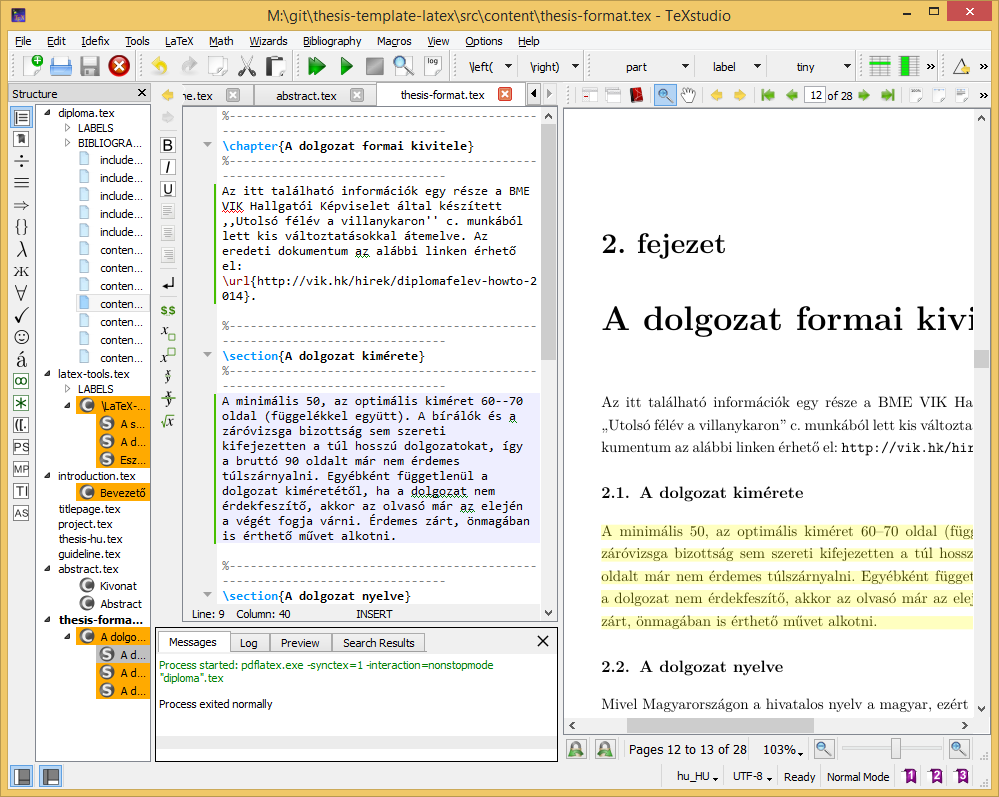
\includegraphics[width=25mm, keepaspectratio]{figures/TeXstudio.png}
\caption{random kép} 
\end{figure}

% Acknowledgements
%~~~~~~~~~~~~~~~~~~~~~~~~~~~~~~~~~~~~~~~~~~~~~~~~~~~~~~~~~~~~~~~~~~~~~~~~~~~~~~~~~~~~~~
% KÖSZONETNYILVÁNÍTÁS

%----------------------------------------------------------------------------
\chapter*{\koszonetnyilvanitas}\addcontentsline{toc}{chapter}{\koszonetnyilvanitas}
%----------------------------------------------------------------------------

Szeretném megköszönni konzulensemnek \textit{Kövesdán Gábor}nak, hogy bármikor kereshettem őt problémáimmal, és akár hétvégén, akár este, segítségemre volt.

Szertném továbbá megköszönni a dolgozatom megírását \textit{támogató cég}nek, hogy rendelkezésmre bocsájtotta az Amazon hozzáférésüket és finanszírozta a Kubernetes klaszter működtetését.

Köszönöm \textit{kollégáimnak, barátaimnak, ismerőseimnek} a felém tanúsított türelmüket és megértésüket, nagyra értékelem, sok teendőt vettek le vállamról.

Az, hogy viszonylag gyorsan tudtam haladni a Schönherz Zoltán kollégiumban tevékenykedő \textit{Kollégiumi Számítástechnikai Kör}ben (KSZK) idők során összegyűjtött tudásomnak köszönhető, hálás vagyok az itt szerzett rengeteg tapasztalatért.

Végül de nem utolsó sorban: rendkívül sok hálával tartozom \textit{Páromnak és családomnak}, hogy türelemmel viselték fáradtságomat, feszültségemet; illetve kíméltek a dolgozatom megírása során.
\vskip 0.5in
\centering
\textbf{Dolgozatom egészen biztosan nem, vagy csak nehezen jöhetett volna támogatásuk nélkül.}


% List of Figures, Tables
%~~~~~~~~~~~~~~~~~~~~~~~~~~~~~~~~~~~~~~~~~~~~~~~~~~~~~~~~~~~~~~~~~~~~~~~~~~~~~~~~~~~~~~
\listoffigures\addcontentsline{toc}{chapter}{\listfigurename}
%\listoftables\addcontentsline{toc}{chapter}{\listtablename}


% Bibliography
%~~~~~~~~~~~~~~~~~~~~~~~~~~~~~~~~~~~~~~~~~~~~~~~~~~~~~~~~~~~~~~~~~~~~~~~~~~~~~~~~~~~~~~
\addcontentsline{toc}{chapter}{\bibname}
\bibliography{bib/bibliography}


% Appendix
%~~~~~~~~~~~~~~~~~~~~~~~~~~~~~~~~~~~~~~~~~~~~~~~~~~~~~~~~~~~~~~~~~~~~~~~~~~~~~~~~~~~~~~
%% FÜGGELÉK

%----------------------------------------------------------------------------
\appendix
%----------------------------------------------------------------------------
\chapter*{\fuggelek}\addcontentsline{toc}{chapter}{\fuggelek}
\setcounter{chapter}{\appendixnumber}
%\setcounter{equation}{0} % a fofejezet-szamlalo az angol ABC 6. betuje (F) lesz
\numberwithin{equation}{section}
\numberwithin{figure}{section}
\numberwithin{lstlisting}{section}
%\numberwithin{tabular}{section}

%----------------------------------------------------------------------------
\section{A TeXstudio felülete}
%----------------------------------------------------------------------------
\begin{figure}[!ht]
\centering
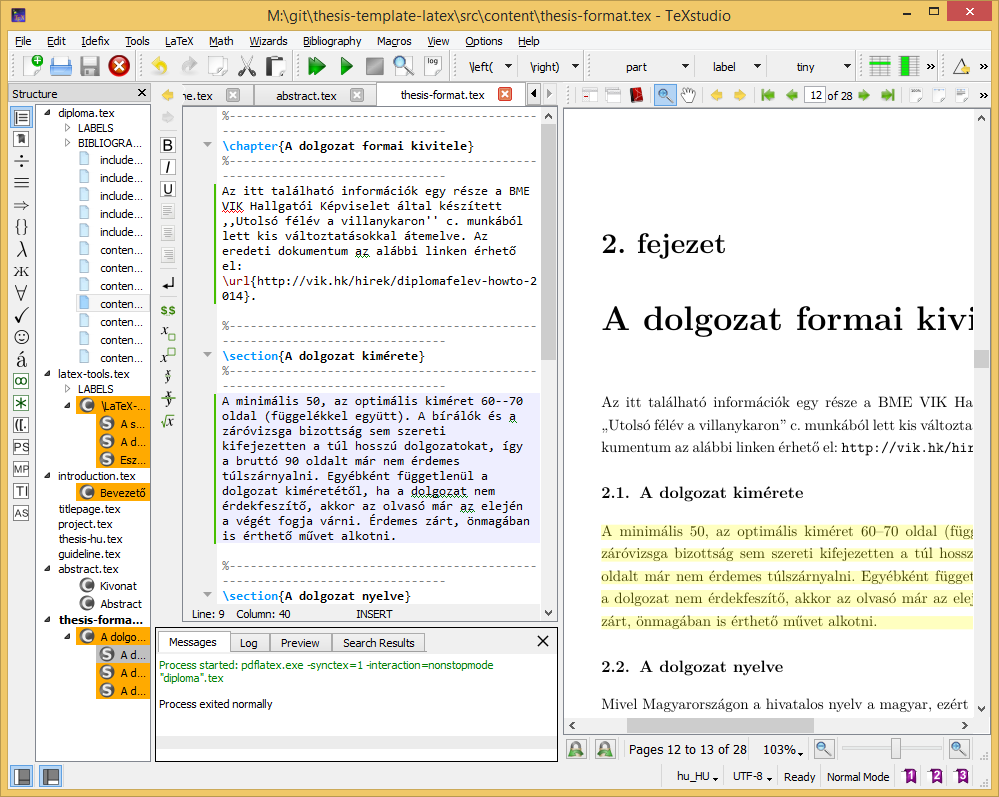
\includegraphics[width=150mm, keepaspectratio]{figures/TeXstudio.png}
\caption{A TeXstudio \LaTeX-szerkesztő.} 
\end{figure}

%----------------------------------------------------------------------------
\clearpage\section{Válasz az ,,Élet, a világmindenség, meg minden'' kérdésére}
%----------------------------------------------------------------------------
A Pitagorasz-tételből levezetve
\begin{align}
c^2=a^2+b^2=42.
\end{align}
A Faraday-indukciós törvényből levezetve
\begin{align}
\rot E=-\frac{dB}{dt}\hspace{1cm}\longrightarrow \hspace{1cm}
U_i=\oint\limits_\mathbf{L}{\mathbf{E}\mathbf{dl}}=-\frac{d}{dt}\int\limits_A{\mathbf{B}\mathbf{da}}=42.
\end{align}


%\label{page:last}
\end{document}
